% Options for packages loaded elsewhere
% Options for packages loaded elsewhere
\PassOptionsToPackage{unicode}{hyperref}
\PassOptionsToPackage{hyphens}{url}
\PassOptionsToPackage{dvipsnames,svgnames,x11names}{xcolor}
%
\documentclass[
  letterpaper,
  DIV=11,
  numbers=noendperiod]{scrreprt}
\usepackage{xcolor}
\usepackage[margin=1.5in,heightrounded]{geometry}
\usepackage{amsmath,amssymb}
\setcounter{secnumdepth}{2}
\usepackage{iftex}
\ifPDFTeX
  \usepackage[T1]{fontenc}
  \usepackage[utf8]{inputenc}
  \usepackage{textcomp} % provide euro and other symbols
\else % if luatex or xetex
  \usepackage{unicode-math} % this also loads fontspec
  \defaultfontfeatures{Scale=MatchLowercase}
  \defaultfontfeatures[\rmfamily]{Ligatures=TeX,Scale=1}
\fi
\usepackage{lmodern}
\ifPDFTeX\else
  % xetex/luatex font selection
\fi
% Use upquote if available, for straight quotes in verbatim environments
\IfFileExists{upquote.sty}{\usepackage{upquote}}{}
\IfFileExists{microtype.sty}{% use microtype if available
  \usepackage[]{microtype}
  \UseMicrotypeSet[protrusion]{basicmath} % disable protrusion for tt fonts
}{}
\makeatletter
\@ifundefined{KOMAClassName}{% if non-KOMA class
  \IfFileExists{parskip.sty}{%
    \usepackage{parskip}
  }{% else
    \setlength{\parindent}{0pt}
    \setlength{\parskip}{6pt plus 2pt minus 1pt}}
}{% if KOMA class
  \KOMAoptions{parskip=half}}
\makeatother
% Make \paragraph and \subparagraph free-standing
\makeatletter
\ifx\paragraph\undefined\else
  \let\oldparagraph\paragraph
  \renewcommand{\paragraph}{
    \@ifstar
      \xxxParagraphStar
      \xxxParagraphNoStar
  }
  \newcommand{\xxxParagraphStar}[1]{\oldparagraph*{#1}\mbox{}}
  \newcommand{\xxxParagraphNoStar}[1]{\oldparagraph{#1}\mbox{}}
\fi
\ifx\subparagraph\undefined\else
  \let\oldsubparagraph\subparagraph
  \renewcommand{\subparagraph}{
    \@ifstar
      \xxxSubParagraphStar
      \xxxSubParagraphNoStar
  }
  \newcommand{\xxxSubParagraphStar}[1]{\oldsubparagraph*{#1}\mbox{}}
  \newcommand{\xxxSubParagraphNoStar}[1]{\oldsubparagraph{#1}\mbox{}}
\fi
\makeatother

\usepackage{color}
\usepackage{fancyvrb}
\newcommand{\VerbBar}{|}
\newcommand{\VERB}{\Verb[commandchars=\\\{\}]}
\DefineVerbatimEnvironment{Highlighting}{Verbatim}{commandchars=\\\{\}}
% Add ',fontsize=\small' for more characters per line
\usepackage{framed}
\definecolor{shadecolor}{RGB}{241,243,245}
\newenvironment{Shaded}{\begin{snugshade}}{\end{snugshade}}
\newcommand{\AlertTok}[1]{\textcolor[rgb]{0.68,0.00,0.00}{#1}}
\newcommand{\AnnotationTok}[1]{\textcolor[rgb]{0.37,0.37,0.37}{#1}}
\newcommand{\AttributeTok}[1]{\textcolor[rgb]{0.40,0.45,0.13}{#1}}
\newcommand{\BaseNTok}[1]{\textcolor[rgb]{0.68,0.00,0.00}{#1}}
\newcommand{\BuiltInTok}[1]{\textcolor[rgb]{0.00,0.23,0.31}{#1}}
\newcommand{\CharTok}[1]{\textcolor[rgb]{0.13,0.47,0.30}{#1}}
\newcommand{\CommentTok}[1]{\textcolor[rgb]{0.37,0.37,0.37}{#1}}
\newcommand{\CommentVarTok}[1]{\textcolor[rgb]{0.37,0.37,0.37}{\textit{#1}}}
\newcommand{\ConstantTok}[1]{\textcolor[rgb]{0.56,0.35,0.01}{#1}}
\newcommand{\ControlFlowTok}[1]{\textcolor[rgb]{0.00,0.23,0.31}{\textbf{#1}}}
\newcommand{\DataTypeTok}[1]{\textcolor[rgb]{0.68,0.00,0.00}{#1}}
\newcommand{\DecValTok}[1]{\textcolor[rgb]{0.68,0.00,0.00}{#1}}
\newcommand{\DocumentationTok}[1]{\textcolor[rgb]{0.37,0.37,0.37}{\textit{#1}}}
\newcommand{\ErrorTok}[1]{\textcolor[rgb]{0.68,0.00,0.00}{#1}}
\newcommand{\ExtensionTok}[1]{\textcolor[rgb]{0.00,0.23,0.31}{#1}}
\newcommand{\FloatTok}[1]{\textcolor[rgb]{0.68,0.00,0.00}{#1}}
\newcommand{\FunctionTok}[1]{\textcolor[rgb]{0.28,0.35,0.67}{#1}}
\newcommand{\ImportTok}[1]{\textcolor[rgb]{0.00,0.46,0.62}{#1}}
\newcommand{\InformationTok}[1]{\textcolor[rgb]{0.37,0.37,0.37}{#1}}
\newcommand{\KeywordTok}[1]{\textcolor[rgb]{0.00,0.23,0.31}{\textbf{#1}}}
\newcommand{\NormalTok}[1]{\textcolor[rgb]{0.00,0.23,0.31}{#1}}
\newcommand{\OperatorTok}[1]{\textcolor[rgb]{0.37,0.37,0.37}{#1}}
\newcommand{\OtherTok}[1]{\textcolor[rgb]{0.00,0.23,0.31}{#1}}
\newcommand{\PreprocessorTok}[1]{\textcolor[rgb]{0.68,0.00,0.00}{#1}}
\newcommand{\RegionMarkerTok}[1]{\textcolor[rgb]{0.00,0.23,0.31}{#1}}
\newcommand{\SpecialCharTok}[1]{\textcolor[rgb]{0.37,0.37,0.37}{#1}}
\newcommand{\SpecialStringTok}[1]{\textcolor[rgb]{0.13,0.47,0.30}{#1}}
\newcommand{\StringTok}[1]{\textcolor[rgb]{0.13,0.47,0.30}{#1}}
\newcommand{\VariableTok}[1]{\textcolor[rgb]{0.07,0.07,0.07}{#1}}
\newcommand{\VerbatimStringTok}[1]{\textcolor[rgb]{0.13,0.47,0.30}{#1}}
\newcommand{\WarningTok}[1]{\textcolor[rgb]{0.37,0.37,0.37}{\textit{#1}}}

\usepackage{longtable,booktabs,array}
\newcounter{none} % for unnumbered tables
\usepackage{calc} % for calculating minipage widths
% Correct order of tables after \paragraph or \subparagraph
\usepackage{etoolbox}
\makeatletter
\patchcmd\longtable{\par}{\if@noskipsec\mbox{}\fi\par}{}{}
\makeatother
% Allow footnotes in longtable head/foot
\IfFileExists{footnotehyper.sty}{\usepackage{footnotehyper}}{\usepackage{footnote}}
\makesavenoteenv{longtable}
\usepackage{graphicx}
\makeatletter
\newsavebox\pandoc@box
\newcommand*\pandocbounded[1]{% scales image to fit in text height/width
  \sbox\pandoc@box{#1}%
  \Gscale@div\@tempa{\textheight}{\dimexpr\ht\pandoc@box+\dp\pandoc@box\relax}%
  \Gscale@div\@tempb{\linewidth}{\wd\pandoc@box}%
  \ifdim\@tempb\p@<\@tempa\p@\let\@tempa\@tempb\fi% select the smaller of both
  \ifdim\@tempa\p@<\p@\scalebox{\@tempa}{\usebox\pandoc@box}%
  \else\usebox{\pandoc@box}%
  \fi%
}
% Set default figure placement to htbp
\def\fps@figure{htbp}
\makeatother





\setlength{\emergencystretch}{3em} % prevent overfull lines

\providecommand{\tightlist}{%
  \setlength{\itemsep}{0pt}\setlength{\parskip}{0pt}}



 


\KOMAoption{captions}{tableheading}
\makeatletter
\@ifpackageloaded{tcolorbox}{}{\usepackage[skins,breakable]{tcolorbox}}
\@ifpackageloaded{fontawesome5}{}{\usepackage{fontawesome5}}
\definecolor{quarto-callout-color}{HTML}{909090}
\definecolor{quarto-callout-note-color}{HTML}{0758E5}
\definecolor{quarto-callout-important-color}{HTML}{CC1914}
\definecolor{quarto-callout-warning-color}{HTML}{EB9113}
\definecolor{quarto-callout-tip-color}{HTML}{00A047}
\definecolor{quarto-callout-caution-color}{HTML}{FC5300}
\definecolor{quarto-callout-color-frame}{HTML}{acacac}
\definecolor{quarto-callout-note-color-frame}{HTML}{4582ec}
\definecolor{quarto-callout-important-color-frame}{HTML}{d9534f}
\definecolor{quarto-callout-warning-color-frame}{HTML}{f0ad4e}
\definecolor{quarto-callout-tip-color-frame}{HTML}{02b875}
\definecolor{quarto-callout-caution-color-frame}{HTML}{fd7e14}
\makeatother
\makeatletter
\@ifpackageloaded{bookmark}{}{\usepackage{bookmark}}
\makeatother
\makeatletter
\@ifpackageloaded{caption}{}{\usepackage{caption}}
\AtBeginDocument{%
\ifdefined\contentsname
  \renewcommand*\contentsname{Table of contents}
\else
  \newcommand\contentsname{Table of contents}
\fi
\ifdefined\listfigurename
  \renewcommand*\listfigurename{List of Figures}
\else
  \newcommand\listfigurename{List of Figures}
\fi
\ifdefined\listtablename
  \renewcommand*\listtablename{List of Tables}
\else
  \newcommand\listtablename{List of Tables}
\fi
\ifdefined\figurename
  \renewcommand*\figurename{Figure}
\else
  \newcommand\figurename{Figure}
\fi
\ifdefined\tablename
  \renewcommand*\tablename{Table}
\else
  \newcommand\tablename{Table}
\fi
}
\@ifpackageloaded{float}{}{\usepackage{float}}
\floatstyle{ruled}
\@ifundefined{c@chapter}{\newfloat{codelisting}{h}{lop}}{\newfloat{codelisting}{h}{lop}[chapter]}
\floatname{codelisting}{Listing}
\newcommand*\listoflistings{\listof{codelisting}{List of Listings}}
\usepackage{amsthm}
\theoremstyle{plain}
\newtheorem{theorem}{Theorem}[chapter]
\theoremstyle{plain}
\newtheorem{corollary}{Corollary}[chapter]
\theoremstyle{plain}
\newtheorem{lemma}{Lemma}[chapter]
\theoremstyle{plain}
\newtheorem{proposition}{Proposition}[chapter]
\theoremstyle{definition}
\newtheorem{exercise}{Exercise}[chapter]
\theoremstyle{definition}
\newtheorem{example}{Example}[chapter]
\theoremstyle{definition}
\newtheorem{definition}{Definition}[chapter]
\theoremstyle{remark}
\AtBeginDocument{\renewcommand*{\proofname}{Proof}}
\newtheorem*{remark}{Remark}
\newtheorem*{solution}{Solution}
\newtheorem{refremark}{Remark}[chapter]
\newtheorem{refsolution}{Solution}[chapter]
\makeatother
\makeatletter
\makeatother
\makeatletter
\@ifpackageloaded{caption}{}{\usepackage{caption}}
\@ifpackageloaded{subcaption}{}{\usepackage{subcaption}}
\makeatother
\usepackage{bookmark}
\IfFileExists{xurl.sty}{\usepackage{xurl}}{} % add URL line breaks if available
\urlstyle{same}
% fallback for those not using the hyperref driver hyperxmp:
\makeatletter
\@ifundefined{xmpquote}{\newcommand{\xmpquote}[1]{#1}}{}
\makeatother
\hypersetup{
  pdftitle={Math 140H --- Honors Calculus I: Lecture Notes},
  pdfauthor={Jan Reimann},
  colorlinks=true,
  linkcolor={blue},
  filecolor={Maroon},
  citecolor={Blue},
  urlcolor={Blue},
  pdfcreator={LaTeX via pandoc}}


\title{Math 140H --- Honors Calculus I: Lecture Notes}
\author{Jan Reimann}
\date{2026-09-20}
\begin{document}
\maketitle

\renewcommand*\contentsname{Table of contents}
{
\setcounter{tocdepth}{1}
\tableofcontents
}

\bookmarksetup{startatroot}

\chapter*{Welcome!}\label{welcome}
\addcontentsline{toc}{chapter}{Welcome!}

\markboth{Welcome!}{Welcome!}

These notes accompany Math 140H, Honors Calculus I, Fall 2026. Each
lecture here corresponds to one class session and covers more or less
the material presented in class, in the same order, so that it can serve
as a compact study reference. HTML ``hardcopies'' of the Jupyter
notebook activities from class are also included. Lecture notes will
generally be available immediately \textbf{after} the corresponding
class session.

State College, Fall 2026

\part{Real Numbers}

\chapter{The Rational Numbers and the Number
Line}\label{the-rational-numbers-and-the-number-line}

\begin{tcolorbox}[enhanced jigsaw, arc=.35mm, bottomrule=.15mm, bottomtitle=1mm, breakable, colback=white, colbacktitle=quarto-callout-note-color!10!white, colframe=quarto-callout-note-color-frame, coltitle=black, left=2mm, leftrule=.75mm, opacityback=0, opacitybacktitle=0.6, rightrule=.15mm, title={Companion reading}, titlerule=0mm, toprule=.15mm, toptitle=1mm]

This lecture corresponds to C\&J §1.1a, together with the neighborhood
definition from §1.1d --- covered a bit early here since we will use it
constantly for the rest of the semester.

\end{tcolorbox}

Calculus is built on the real numbers, so before we can talk about
limits, derivatives, or integrals we need to understand exactly what a
real number \emph{is} --- and, just as importantly, why the rational
numbers alone are not enough. This lecture makes that precise: we recall
how the natural numbers extend to the rationals, set up the number line,
and then prove that a length as ordinary as the hypotenuse of a simple
right triangle cannot be a rational number at all.

\section{From Counting to Measuring}\label{from-counting-to-measuring}

There are two major uses for numbers: \textbf{counting} and
\textbf{measuring}. The natural numbers \(\mathbb{N}= \{1,2,3,\dots\}\)
are the tool for counting --- abstract symbols for how many elements are
in a collection, stripped of any reference to what is actually being
counted. They come equipped with addition and multiplication satisfying
a short list of familiar rules.

\begin{refremark}
For all natural numbers \(a,b,c\):

\begin{itemize}
\tightlist
\item
  \(a+b=b+a\) and \(ab=ba\)   (commutative laws)
\item
  \(a+(b+c)=(a+b)+c\) and \(a(bc)=(ab)c\)   (associative laws)
\item
  \(a(b+c)=ab+ac\)   (distributive law)
\item
  \(a+c=b+c \;\Rightarrow\; a=b\)   (cancellation law)
\end{itemize}

These are the \emph{rules} of arithmetic, not its \emph{content} ---
everything else in this course is built on top of them, and we will not
dwell on them further.

\label{rem-arithmetic-laws}

\end{refremark}

Natural numbers can be added and multiplied, but not always subtracted
or divided. There is no natural number \(a\) with \[
5+a=2,
\] so subtraction is not always possible in \(\mathbb{N}\). Extending
\(\mathbb{N}\) to the \textbf{integers}
\(\mathbb{Z}= \{\dots,-2,-1,0,1,2,\dots\}\) fixes this: now
\(5+(-3)=2\).

In \(\mathbb{Z}\), we still cannot always divide: there is no integer
\(b\in\mathbb{Z}\) with \[
5\cdot b = 2 .
\] Extending \(\mathbb{Z}\) to the \textbf{rational numbers} fixes this
in turn.

\begin{definition}[]\protect\hypertarget{def-rational-number}{}\label{def-rational-number}

\hfill\break
A \textbf{rational number} is a number that can be written as \(p/q\)
where \(p,q\in\mathbb{Z}\) and \(q\neq 0\). Every rational number has a
unique representation \(p/q\) with \(q>0\) and \(\gcd(p,q)=1\) (no
common factor larger than \(1\)); we call this representation \textbf{in
lowest terms}.

\end{definition}

Within \(\mathbb{Q}\), all four rational operations --- addition,
subtraction, multiplication, and division (except by \(0\)) --- can be
carried out freely, and they obey exactly the same laws as in
Remark~\ref{rem-arithmetic-laws}. In this precise sense, \(\mathbb{Q}\)
is the smallest extension of the natural numbers in which counting-type
arithmetic becomes measuring-type arithmetic.

\section{The Number Line}\label{the-number-line}

To turn numbers into geometry, fix a line \(L\), a point \(O\) on it
called the \textbf{origin}, and a second point \(I\) to the right of
\(O\); the segment \(OI\) serves as our unit scale for measuring --- a
``prototype meter.'' The direction from \(O\) to \(I\) is called
\textbf{positive}.

Every point on \(L\) is now uniquely determined by two pieces of
information: its \textbf{distance} from \(O\), and its
\textbf{direction} (left or right) from \(O\). For example, the point at
distance \(\tfrac12\) in the positive direction represents the rational
number \(\tfrac12\); the point at distance \(2\) in the positive
direction represents \(2\).

\begin{definition}[]\protect\hypertarget{def-absolute-value}{}\label{def-absolute-value}

\hfill\break
The distance of a number \(x\) from the origin is written \(|x|\) and
called the \textbf{absolute value} of \(x\): \[
|x| \;=\; \begin{cases} \phantom{-}x & x \ge 0 \\ -x & x < 0. \end{cases}
\] Note \(|x|\ge 0\) always, with equality only when \(x=0\).

\end{definition}

Every rational point can in fact be \emph{constructed}, not just
described: to locate \(p/q\) on \(L\) with ruler and compass, construct
a subdivision of the segment \(OI\) into \(q\) equal parts, then extend
the part closest to \(O\), \(p\) times. We will identify each rational
number with its representation on \(L\).

\section{Distances and Intervals}\label{distances-and-intervals}

For \(x,y\in L\), the number \(|x-y|\) is the \textbf{distance between
\(x\) and \(y\)}. Observe: if \(x,y\in\mathbb{Q}\), then
\(|x-y|\in\mathbb{Q}\) as well --- distances between rational points are
themselves rational.

\begin{definition}[]\protect\hypertarget{def-interval}{}\label{def-interval}

\hfill\break
For \(a<b\), the \textbf{interval} between \(a\) and \(b\) comes in four
flavors:

\begin{itemize}
\tightlist
\item
  open:   \((a,b) := \{x : a<x<b\}\)   (both endpoints excluded)
\item
  closed:   \([a,b] := \{x : a\le x\le b\}\)   (both endpoints included)
\item
  half-open:   \([a,b) := \{x: a \le x < b\}\) and
  \((a,b] := \{x : a< x \le b\}\)
\end{itemize}

\end{definition}

\begin{definition}[]\protect\hypertarget{def-neighborhood}{}\label{def-neighborhood}

\hfill\break
Given a number \(a\) and \(\varepsilon>0\), the
\textbf{\(\varepsilon\)-neighborhood of \(a\)} is the open interval \[
\{y : |y-a| < \varepsilon\} = (a-\varepsilon, a+\varepsilon),
\] i.e.~the set of points less than \(\varepsilon\) away from \(a\).

\end{definition}

We will meet \(\varepsilon\)-neighborhoods constantly once we get to
limits --- keep this definition close by.

\subsection{Density}\label{density}

\begin{proposition}[]\protect\hypertarget{prp-density}{}\label{prp-density}

\hfill\break
Between any two distinct rational numbers \(a<b\) there is another
rational number \(c\) with \(a<c<b\). Consequently, between \(a\) and
\(b\) there are infinitely many rational numbers.

\end{proposition}

\begin{proof}
Let \(c=\dfrac{a+b}{2}\). Since \(a,b\in\mathbb{Q}\) and \(\mathbb{Q}\)
is closed under addition and division by \(2\), \(c\in\mathbb{Q}\); and
since \(a<b\), averaging gives \(a<c<b\).

Now repeat the argument on the pair \(a,c\) to get a rational number
strictly between \(a\) and \(c\), hence strictly between \(a\) and
\(b\). Doing this again and again produces infinitely many rational
numbers between \(a\) and \(b\).
\end{proof}

We say the rationals are \textbf{dense} on the number line: no matter
how closely you look, you will always find another one.

\section{Incommensurable Lengths}\label{sec-incommensurable}

Given how constructible and how dense \(\mathbb{Q}\) is, a natural
question arises: is there anything ``left in between'' the rational
numbers? Are there any \emph{gaps}? Clearly, such a gap could not itself
be an interval --- density rules that out, since any interval of
positive length contains infinitely many rational points. If a gap
exists at all, it can only be a single missing point.

\begin{refremark}
The discovery that not every length is a rational multiple of a chosen
unit is due to the school of Pythagoras, in the fifth or sixth century
BCE. Consider a right triangle with both legs of length \(1\); by the
Pythagorean theorem, its hypotenuse \(a\) satisfies \[
1^2+1^2 = a^2 = 2,
\] and \(a\) can certainly be constructed with ruler and compass. The
theorem below shows this length cannot be written as \(p/q\) for
integers \(p,q\) --- the hypotenuse and the legs of this triangle are,
in the language of the ancients, \textbf{incommensurable}: there is no
common unit of which both are integer multiples.

\label{rem-pythagoras}

\end{refremark}

\begin{theorem}[]\protect\hypertarget{thm-sqrt2-irrational}{}\label{thm-sqrt2-irrational}

\hfill\break
There is no rational number \(x\) with \(x^2=2\). Equivalently,
\(\sqrt2 \notin \mathbb{Q}\).

\end{theorem}

\begin{proof}
Suppose, toward a contradiction, that \(\sqrt2 = p/q\) for integers
\(p,q\) with \(q\neq 0\) and \(\gcd(p,q)=1\) (i.e.~\(p/q\) is in lowest
terms).

\begin{enumerate}
\def\labelenumi{\arabic{enumi}.}
\tightlist
\item
  Square both sides and clear the denominator: \(p^2 = 2q^2\).
\item
  Conclude that \(p^2\) is even --- if \(p\) were odd, \(p^2\) would be
  odd, but \(p^2=2q^2\) is even. Write \(p=2r\) for some integer \(r\).
\item
  Substitute \(p=2r\) into the equation from Step 1 and simplify to get
  an equation for \(q^2\) in terms of \(r\):
  \((2r)^2 = 2q^2 \;\Rightarrow\; 4r^2 = 2q^2 \;\Rightarrow\; q^2 = 2r^2\).
\item
  Conclude that \(q\) is also even, by the same reasoning as in Step 2.
\item
  Steps 2 and 4 show that \(2\) divides both \(p\) and \(q\). This
  contradicts \(\gcd(p,q)=1\), which we assumed when we wrote \(p/q\) in
  lowest terms.
\item
  Conclude: \(\sqrt2\) is irrational --- no integers \(p,q\) satisfy
  \(\sqrt2=p/q\), so \(\sqrt2 \notin \mathbb{Q}\).
\end{enumerate}

\end{proof}

\begin{exercise}[]\protect\hypertarget{exr-}{}\label{exr-}

Adapt the proof of Theorem~\ref{thm-sqrt2-irrational} to show that
\(\sqrt3\) is irrational. Then try to see where the argument would break
if you attempted the same proof for \(\sqrt4\) --- since \(\sqrt4=2\) is
certainly rational, something in the argument \emph{must} fail. Where,
exactly?

\end{exercise}

\section{Summary}\label{summary}

\begin{itemize}
\tightlist
\item
  The rationals \(\mathbb{Q}\) satisfy all the usual laws of arithmetic
  (Remark~\ref{rem-arithmetic-laws}) and are \textbf{dense}: between any
  two rationals lies another (Proposition~\ref{prp-density}).
\item
  Distances \(|x-y|\), intervals, and \(\varepsilon\)-neighborhoods
  (Definition~\ref{def-interval}, Definition~\ref{def-neighborhood})
  give us the basic vocabulary for talking about ``closeness'' on the
  number line --- vocabulary we will lean on heavily once limits arrive.
\item
  Density notwithstanding, \(\mathbb{Q}\) does not exhaust the number
  line: Theorem~\ref{thm-sqrt2-irrational} exhibits an ordinary,
  constructible length that is not a rational number.
\item
  The rationals therefore leave \emph{gaps} in the line. Lecture 2
  closes these gaps rigorously, using \textbf{nested intervals} to
  construct the real numbers.
\end{itemize}

\chapter{The Real Numbers via Nested
Intervals}\label{the-real-numbers-via-nested-intervals}

\begin{tcolorbox}[enhanced jigsaw, arc=.35mm, bottomrule=.15mm, bottomtitle=1mm, breakable, colback=white, colbacktitle=quarto-callout-note-color!10!white, colframe=quarto-callout-note-color-frame, coltitle=black, left=2mm, leftrule=.75mm, opacityback=0, opacitybacktitle=0.6, rightrule=.15mm, title={Companion reading}, titlerule=0mm, toprule=.15mm, toptitle=1mm]

This lecture corresponds to C\&J §1.1b--c.

\end{tcolorbox}

Last time we found a gap: the length \(\sqrt2\) is constructible with
ruler and compass, yet Theorem~\ref{thm-sqrt2-irrational} shows it is
not a rational number. So what \emph{is} \(\sqrt2\), as a number? We are
used to describing such quantities through infinite decimal expansions,
e.g. \[
\pi = 3.1415926\ldots,
\] but so far this is just a string of digits --- it is not clear what
it \emph{means} mathematically. The key idea of this lecture is that an
infinite decimal (or any other description of an irrational number) is
really a recipe for \textbf{approximating} a point by rational numbers,
to any desired degree of accuracy. We make this precise using shrinking
intervals with rational endpoints.

\section{Nested Intervals}\label{nested-intervals}

Suppose \(x\) is a point on the number line that we want to pin down
using only rational numbers. Start with any closed interval
\(I_1 = [a_1,b_1]\) with \(a_1,b_1\in\mathbb{Q}\) and
\(a_1 \le x \le b_1\). Now choose a subinterval
\(I_2 = [a_2,b_2] \subseteq I_1\) that still contains \(x\): \[
a_1 \le a_2 \le x \le b_2 \le b_1,
\] for instance by splitting \(I_1\) in half and keeping whichever half
contains \(x\). Repeating this forever produces a chain \[
I_1 \supseteq I_2 \supseteq I_3 \supseteq \cdots, \qquad x \in I_n \text{ for every } n.
\] For this to genuinely \emph{pin down} \(x\) --- rather than just
hover near it --- we need one more ingredient: the intervals must shrink
all the way down to a point.

\begin{definition}[]\protect\hypertarget{def-nested-intervals}{}\label{def-nested-intervals}

\hfill\break
A \textbf{nested sequence of closed intervals with rational endpoints}
is a sequence \(I_n = [a_n,b_n]\), \(n=1,2,3,\dots\), with
\(a_n,b_n\in\mathbb{Q}\), such that

\begin{enumerate}
\def\labelenumi{\arabic{enumi}.}
\tightlist
\item
  \(I_1 \supseteq I_2 \supseteq I_3 \supseteq \cdots\), and
\item
  the lengths \(|I_n| := b_n - a_n\) tend to \(0\) as \(n\to\infty\):
  for every \(\varepsilon>0\) there is an \(N\) such that
  \(|I_n| < \varepsilon\) for all \(n \ge N\).
\end{enumerate}

\end{definition}

\begin{proposition}[]\protect\hypertarget{prp-nested-unique}{}\label{prp-nested-unique}

\hfill\break
If a nested sequence of closed intervals \((I_n)\) contains a point in
every \(I_n\), that point is unique: there is at most one \(x\) with
\(x\in I_n\) for all \(n\).

\end{proposition}

\begin{proof}
Suppose \(x\) and \(y\) both lie in every \(I_n\), and toward a
contradiction suppose \(x\neq y\). Let \(\varepsilon_0 = |x-y| > 0\).
Since \(|I_n|\to 0\), there is some \(n\) with
\(|I_n| < \varepsilon_0\). But \(x,y\in I_n\) means
\(|x-y| \le |I_n| < \varepsilon_0 = |x-y|\), which is absurd. Hence
\(x=y\).
\end{proof}

So a nested sequence of intervals can ``address'' at most one point ---
and, geometrically, every point \(x\) on the line does arise this way:

\begin{theorem}[]\protect\hypertarget{thm-real-nested-intervals}{}\label{thm-real-nested-intervals}

\hfill\break
Every real number \(x\) is the unique point contained in every interval
of some nested sequence of closed intervals with rational endpoints.

\end{theorem}

\begin{proof}
Uniqueness is Proposition~\ref{prp-nested-unique}. For existence, pick
any rational bracket \(I_1=[a_1,b_1]\) with \(a_1 \le x \le b_1\), and
repeatedly bisect: given \(I_n=[a_n,b_n]\), let
\(m_n = \tfrac{a_n+b_n}{2}\) (rational, since \(a_n,b_n\in\mathbb{Q}\)),
and set \[
I_{n+1} = \begin{cases} [a_n,m_n] & \text{if } x \le m_n \\ [m_n,b_n] & \text{if } x > m_n. \end{cases}
\] Then \(x\in I_{n+1}\subseteq I_n\) and \(|I_{n+1}| = |I_n|/2\), so
\(|I_n| = |I_1|/2^{n-1} \to 0\). This is a nested sequence of closed
intervals with rational endpoints containing \(x\).
\end{proof}

In this sense, every real number can be described --- completely and
unambiguously --- by an infinite sequence of rational numbers (the
endpoints \(a_n,b_n\)).

\section{The Nested Interval Axiom}\label{the-nested-interval-axiom}

The construction above starts from a real number \(x\) and produces a
nested sequence around it. What about the converse: if we are simply
\emph{handed} a nested sequence of closed intervals with rational
endpoints, must there be a point in \(\bigcap_n I_n\) at all?

For \textbf{open} intervals, the answer is no: \(I_n = (0, \tfrac1n)\)
satisfies \(I_1 \supseteq I_2
\supseteq \cdots\) and \(|I_n| = \tfrac1n \to 0\), yet no point lies in
every \(I_n\) --- any candidate \(x>0\) fails once \(n > 1/x\), and
\(x=0\) is excluded from every \(I_n\) by openness.

For \textbf{closed} intervals, this is far less obvious, and cannot be
deduced from the algebraic properties of \(\mathbb{Q}\) alone (after
all, \(\mathbb{Q}\) itself has a gap at \(\sqrt2\)). We take it as a
basic postulate about the number line.

\begin{tcolorbox}[enhanced jigsaw, arc=.35mm, bottomrule=.15mm, bottomtitle=1mm, breakable, colback=white, colbacktitle=quarto-callout-important-color!10!white, colframe=quarto-callout-important-color-frame, coltitle=black, left=2mm, leftrule=.75mm, opacityback=0, opacitybacktitle=0.6, rightrule=.15mm, title={Axiom (Nested Interval Property)}, titlerule=0mm, toprule=.15mm, toptitle=1mm]

If \(I_1 \supseteq I_2 \supseteq I_3 \supseteq \cdots\) is a nested
sequence of closed intervals with rational endpoints, then \[
\bigcap_{n\in\mathbb{N}} I_n \neq \emptyset,
\] i.e.~there is a point \(x\) contained in every \(I_n\).

\end{tcolorbox}

This is a genuine \textbf{axiom}: a basic postulate we accept without
proof, rather than a consequence of things we already know. Together
with Proposition~\ref{prp-nested-unique}, it guarantees that no gaps
exist on the number line --- every nested sequence of rational brackets
zeroes in on exactly one real number, no more and no less. This
completeness of the number line is fundamental for everything that
follows in this course; we will meet it again, in other guises, once we
get to limits.

\section{Decimal Expansions}\label{decimal-expansions}

Decimal expansions are simply a very concrete, systematic way of
producing a nested sequence of intervals --- one that subdivides by tens
at every step.

\begin{definition}[]\protect\hypertarget{def-decimal-expansion}{}\label{def-decimal-expansion}

\hfill\break
Let \(x\) be a point on the number line. Set \[
c_0 := \lfloor x \rfloor,
\] the greatest integer with \(c_0 \le x \le c_0+1\), and
\(I_0 = [c_0, c_0+1]\), so \(|I_0|=1\).

Divide \(I_0\) into ten equal parts using the points
\(c_0+\tfrac1{10}, c_0+\tfrac2{10},\dots,
c_0+\tfrac9{10}\), and let \(c_1\in\{0,1,\dots,9\}\) be the digit with
\[
c_0 + \frac{c_1}{10} \;\le\; x \;\le\; c_0 + \frac{c_1}{10} + \frac{1}{10},
\] and set \(I_1\) to be this interval, so \(|I_1| = \tfrac1{10}\).

Iterating, having chosen digits \(c_1,\dots,c_{n-1}\in\{0,\dots,9\}\),
subdivide \(I_{n-1}\) into ten equal parts and let
\(c_n\in\{0,\dots,9\}\) be the digit with \[
c_0 + \frac{c_1}{10} + \cdots + \frac{c_n}{10^n} \;\le\; x \;\le\; c_0 + \frac{c_1}{10} + \cdots +
\frac{c_n}{10^n} + \frac{1}{10^n},
\] and let \(I_n\) be this interval, so \(|I_n| = 10^{-n}\).

\end{definition}

By construction \((I_n)_{n\ge0}\) is exactly a nested sequence of closed
intervals with rational endpoints in the sense of
Definition~\ref{def-nested-intervals}:
\(I_0\supseteq I_1\supseteq I_2\supseteq\cdots\), each contains \(x\),
and \(|I_n| = 10^{-n} \to 0\). We abbreviate this whole sequence by
writing \[
x = c_0 + 0.c_1c_2c_3\ldots,
\] the \textbf{decimal expansion} of \(x\) --- a notational shortcut for
the nested intervals, not a new kind of number. (Careful when \(c_0<0\):
the digits after the point are still \emph{added} to \(c_0\). For
instance \(x=-2.75\) has \(c_0 = \lfloor -2.75\rfloor = -3\) and
\(x = -3 + 0.25\), not \(-3-0.25\).)

Combining Definition~\ref{def-decimal-expansion} with
Proposition~\ref{prp-nested-unique} and the Nested Interval Axiom:

\begin{itemize}
\tightlist
\item
  Every real number has an (infinite) decimal expansion.
\item
  Conversely, every such expansion --- i.e.~every choice of
  \(c_0\in\mathbb{Z}\) and digits \(c_1,c_2,\dots\in\{0,\dots,9\}\) ---
  is a nested sequence of closed intervals with rational endpoints, so
  by the axiom it defines a real number.
\end{itemize}

\begin{tcolorbox}[enhanced jigsaw, arc=.35mm, bottomrule=.15mm, bottomtitle=1mm, breakable, colback=white, colbacktitle=quarto-callout-warning-color!10!white, colframe=quarto-callout-warning-color-frame, coltitle=black, left=2mm, leftrule=.75mm, opacityback=0, opacitybacktitle=0.6, rightrule=.15mm, title={Decimal expansions are not always unique}, titlerule=0mm, toprule=.15mm, toptitle=1mm]

Some real numbers have \emph{two} decimal expansions: for instance \[
1.000\ldots = 0.999\ldots.
\]

\end{tcolorbox}

\begin{exercise}[]\protect\hypertarget{exr-decimal-not-unique}{}\label{exr-decimal-not-unique}

Why does \(1.000\ldots = 0.999\ldots\)? (Hint: what would
\(1 - 0.999\ldots\) have to be, if it were positive?) More generally,
can you characterize \emph{exactly} which real numbers have two decimal
expansions?

\end{exercise}

\begin{solution}
If \(1 - 0.999\ldots = \delta > 0\), then \(\delta\) would have to be
smaller than \(10^{-n}\) for every \(n\) (since
\(0.\underbrace{9\cdots9}_{n} = 1 - 10^{-n}\) already exceeds
\(1-\delta\)), forcing \(\delta=0\) --- contradiction. So the two
expansions name the same point.

In general, a real number has two decimal expansions exactly when it is
a \textbf{terminating} decimal, i.e.~of the form \(m/10^n\) for some
\(m\in\mathbb{Z}\), \(n\ge0\): one expansion ends in all \(0\)'s, the
other in all \(9\)'s. Every other real number has a unique decimal
expansion.
\end{solution}

\section{Other Bases}\label{other-bases}

Nothing in Definition~\ref{def-decimal-expansion} is special about the
number \(10\) --- we could subdivide each interval into any number
\(p>1\) of equal parts instead of ten, producing digits
\(c_i \in \{0,1,\dots,p-1\}\) and a \textbf{base-\(p\) (or \(p\)-ary)
expansion} of \(x\).

The case \(p=2\), the \textbf{binary expansion}, is exactly the
bisection procedure from the proof of
Theorem~\ref{thm-real-nested-intervals}: at each step we only need to
decide whether \(x\) lies in the lower or upper half of the current
interval.

\begin{example}[]\protect\hypertarget{exm-binary-expansion}{}\label{exm-binary-expansion}

\hfill\break
Let's find the first three binary digits of \(x=0.76\). Start with
\(I_0=[0,1]\), so \(c_0=0\).

\begin{itemize}
\tightlist
\item
  Midpoint \(0.5\): since \(0.76 \ge 0.5\), digit \(c_1=1\) and
  \(I_1=[0.5,1]\).
\item
  Midpoint \(0.75\): since \(0.76 \ge 0.75\), digit \(c_2=1\) and
  \(I_2=[0.75,1]\).
\item
  Midpoint \(0.875\): since \(0.76 < 0.875\), digit \(c_3=0\) and
  \(I_3=[0.75,0.875]\).
\end{itemize}

So \(0.76 = 0.110\ldots\) in base \(2\).

\end{example}

\begin{exercise}[]\protect\hypertarget{exr-other-base-expansions}{}\label{exr-other-base-expansions}

Find the first three fractional digits of the base-\(2\) expansion of
\(x=0.3\), and the first three fractional digits of the base-\(3\)
expansion of \(x=0.76\).

\end{exercise}

\section{Summary}\label{summary-1}

\begin{itemize}
\tightlist
\item
  A \textbf{nested sequence of closed intervals with rational endpoints}
  (Definition~\ref{def-nested-intervals}) can contain at most one point
  (Proposition~\ref{prp-nested-unique}), and every real number arises as
  the unique point of some such sequence
  (Theorem~\ref{thm-real-nested-intervals}).
\item
  The converse --- that every nested sequence of closed intervals with
  rational endpoints \emph{does} contain a point --- is not provable
  from what came before; it is the \textbf{Nested Interval Axiom}, the
  basic postulate that guarantees there are no gaps in the number line.
\item
  \textbf{Decimal expansions} (Definition~\ref{def-decimal-expansion})
  are the special case of base-\(10\) subdivision; every real number has
  one, though numbers of the form \(m/10^n\) have exactly two
  (Exercise~\ref{exr-decimal-not-unique}).
\item
  The same construction works in any base \(p>1\), giving \(p\)-ary
  expansions; base \(2\) is exactly the bisection algorithm behind
  Theorem~\ref{thm-real-nested-intervals}.
\end{itemize}

\chapter{Jupyter Activity: p-ary
Expansions}\label{jupyter-activity-p-ary-expansions}

Math 140H, Honors Calculus I

\section{Before we start: how to use a Jupyter
notebook}\label{before-we-start-how-to-use-a-jupyter-notebook}

This is the first notebook of the semester, so we start a quick
orientation:

\begin{itemize}
\tightlist
\item
  A notebook is a sequence of \textbf{cells}. This text lives in a
  \emph{markdown cell} (formatted text); cells with \texttt{code} in the
  toolbar are \emph{code cells} (Python).
\item
  Click a cell and press \textbf{Shift+Enter} to run it and move to the
  next one. Code cells must be run in order the first time through, top
  to bottom --- a later cell may use a function or variable that an
  earlier cell defined.
\item
  If something breaks, it is often because a cell was skipped or run
  twice out of order. Use the menu command \emph{Run All} (or
  \emph{Restart Kernel and Run All}) to run the whole notebook cleanly
  from the top.
\item
  You do \textbf{not} need to know Python already. Every function below
  is commented line by line --- read the comments (the lines starting
  with \texttt{\#}) as a description of the math, and the code as one
  particular way of writing it down.
\end{itemize}

\subsection{Code cells}\label{code-cells}

You can think of a code cell very much like a fancy calculator. Move to
the next cell an run it.

\begin{Shaded}
\begin{Highlighting}[]
\DecValTok{16}\OperatorTok{+}\NormalTok{(}\DecValTok{53}\OperatorTok{*}\FloatTok{8.7777}\OperatorTok{{-}}\DecValTok{128}\NormalTok{)}
\end{Highlighting}
\end{Shaded}

\begin{verbatim}
353.2181
\end{verbatim}

Careful: In Python, exponentiation is \texttt{**}, not \texttt{\^{}}.

\begin{Shaded}
\begin{Highlighting}[]
\DecValTok{2}\OperatorTok{**}\DecValTok{4}
\end{Highlighting}
\end{Shaded}

\begin{verbatim}
16
\end{verbatim}

\begin{Shaded}
\begin{Highlighting}[]
\DecValTok{2}\OperatorTok{\^{}}\DecValTok{4}
\end{Highlighting}
\end{Shaded}

\begin{verbatim}
6
\end{verbatim}

\texttt{\^{}} in Python is the operation called \texttt{bitwise\ XOR};
that explains the strange result above.

We will learn more about Jupyter notebooks (and a little bit more about
Python) in the course of this semester. Today, we will simply experiment
a bit with pre-defined Python function that converts rational numbers to
\(p\)-ary expansions. Go ahead and run the cells below one after the
other (do not forget to read the text inbetween.)

\begin{center}\rule{0.5\linewidth}{0.5pt}\end{center}

\section{Importing Python modules}\label{importing-python-modules}

A lot functionality in Python is provided by \emph{modules}. The
following cell loads the modules we need for this notebook.

\begin{Shaded}
\begin{Highlighting}[]
\CommentTok{\# We import three tools before doing anything else:}
\CommentTok{\#}
\CommentTok{\#   math     {-}{-} the standard library module with math.floor(y), the greatest integer \textless{}= y.}
\CommentTok{\#               (We need floor of *exact fractions*, not of floating{-}point approximations {-}{-}}
\CommentTok{\#               see the note below.)}
\CommentTok{\#   Fraction {-}{-} from the \textquotesingle{}fractions\textquotesingle{} module. A Fraction stores a rational number as an exact}
\CommentTok{\#               numerator/denominator pair, e.g. Fraction(1, 3) is *exactly* one third, forever.}
\CommentTok{\#               This matters a lot here: a computer\textquotesingle{}s ordinary decimal numbers (called \textquotesingle{}floats\textquotesingle{})}
\CommentTok{\#               are themselves binary approximations, so 1/3 as a float is already slightly wrong,}
\CommentTok{\#               and the tiny error would snowball after enough steps of the algorithm below.}
\CommentTok{\#               Using Fraction means every digit we compute is provably correct, not just close.}
\CommentTok{\#   numpy    {-}{-} imported as \textquotesingle{}np\textquotesingle{} by convention. We use it only to store the list of digits we}
\CommentTok{\#               compute as a numpy array, which is a convenient container for a sequence of numbers.}
\ImportTok{import}\NormalTok{ math}
\ImportTok{from}\NormalTok{ fractions }\ImportTok{import}\NormalTok{ Fraction}
\ImportTok{import}\NormalTok{ numpy }\ImportTok{as}\NormalTok{ np}
\end{Highlighting}
\end{Shaded}

The cells below show the advantage of the \texttt{Fraction} function:

\begin{Shaded}
\begin{Highlighting}[]
\DecValTok{1}\OperatorTok{/}\DecValTok{2}\OperatorTok{+}\DecValTok{1}\OperatorTok{/}\DecValTok{3}   \CommentTok{\# will use decimal expansions}
\end{Highlighting}
\end{Shaded}

\begin{verbatim}
0.8333333333333333
\end{verbatim}

\begin{Shaded}
\begin{Highlighting}[]
\NormalTok{Fraction(}\DecValTok{1}\NormalTok{,}\DecValTok{2}\NormalTok{)}\OperatorTok{+}\NormalTok{Fraction(}\DecValTok{1}\NormalTok{,}\DecValTok{3}\NormalTok{)   }\CommentTok{\# will preserve the precise fraction representation}
\end{Highlighting}
\end{Shaded}

\begin{verbatim}
Fraction(5, 6)
\end{verbatim}

\section{\texorpdfstring{From a rational number to its \emph{p}-ary
expansion}{From a rational number to its p-ary expansion}}\label{from-a-rational-number-to-its-p-ary-expansion}

We generalize the nested interval construction to base \(p\): given
\(x\), set \[
c_0 := \lfloor x \rfloor,
\] and then repeatedly zoom in. Having peeled off
\(c_0,c_1,\dots,c_{n-1}\), look at what is left over,

\[
r_{n-1} \;=\; x - c_0 - \frac{1}{p}c_1 - \cdots - \frac{1}{p^{n-1}}c_{n-1} \;\in [0, p^{-(n-1)}),
\]

multiply it by \(p^{n-1}\) so it lands back in \([0,1)\), and read off
the next digit as the integer part of \(p\) times that:

\[
c_n = \lfloor p \cdot (p^{n-1} r_{n-1}) \rfloor.
\] (Multiplying by \(p\) here means zooming in by a factor of \(p\).)

The function below does exactly this, but it tracks the \emph{rescaled}
remainder (called \texttt{remainder} in the code, always kept in
\([0,1)\)) rather than \(r_{n-1}\) itself, since that is what you
actually multiply by \(p\) at each step:

\begin{enumerate}
\def\labelenumi{\arabic{enumi}.}
\tightlist
\item
  \texttt{remainder\ =\ x\ -\ floor(x)}, the fractional part of \(x\),
  in \([0,1)\).
\item
  Repeat: multiply \texttt{remainder} by \texttt{p}. Its integer part is
  the next digit; subtract that integer part off, leaving a new
  \texttt{remainder} back in \([0,1)\), and go again.
\end{enumerate}

\begin{Shaded}
\begin{Highlighting}[]
\KeywordTok{def}\NormalTok{ rational\_to\_p\_ary(x, p, max\_digits}\OperatorTok{=}\DecValTok{50}\NormalTok{):}
    \CommentTok{"""}
\CommentTok{    Compute the base{-}p expansion of a rational number x.}

\CommentTok{    Parameters}
\CommentTok{    {-}{-}{-}{-}{-}{-}{-}{-}{-}{-}}
\CommentTok{    x : Fraction, int, or a string like "7/12"}
\CommentTok{        The rational number to expand. (Do NOT pass a plain float such as 0.76 {-}{-} floats are}
\CommentTok{        already binary approximations, so we would be expanding the wrong number. Use}
\CommentTok{        Fraction(76, 100) instead. See the discussion above.)}
\CommentTok{    p : int}
\CommentTok{        The base, an integer \textgreater{} 1 (p = 2 for binary, p = 10 for the usual decimal expansion, ...).}
\CommentTok{    max\_digits : int, optional (default = 50)}
\CommentTok{        how many fractional digits to compute }
\CommentTok{        }
\CommentTok{    Returns}
\CommentTok{    {-}{-}{-}{-}{-}{-}{-}}
\CommentTok{    integer\_part : int}
\CommentTok{        c\_0, the integer part of x (i.e. floor(x)).}
\CommentTok{    digits : numpy array of int}
\CommentTok{        The fractional digits c\_1, c\_2, c\_3, ... that were computed, in order.}
\CommentTok{    repeat\_start : int or None}
\CommentTok{        If the expansion is eventually periodic, the index (0{-}based, into \textasciigrave{}digits\textasciigrave{}) where the}
\CommentTok{        repeating block begins. If the expansion terminates exactly (all later digits are 0),}
\CommentTok{        this is None.}
\CommentTok{    """}
    \ControlFlowTok{if} \KeywordTok{not} \BuiltInTok{isinstance}\NormalTok{(p, }\BuiltInTok{int}\NormalTok{) }\KeywordTok{or}\NormalTok{ p }\OperatorTok{\textless{}=} \DecValTok{1}\NormalTok{:}
        \ControlFlowTok{raise} \PreprocessorTok{ValueError}\NormalTok{(}\StringTok{"the base p must be an integer greater than 1"}\NormalTok{)}

    \CommentTok{\# Convert x to an exact fraction, no matter what form it was given in.}
\NormalTok{    x }\OperatorTok{=}\NormalTok{ Fraction(x)}

    \CommentTok{\# Step 1: peel off the integer part c\_0 = floor(x). What remains, x {-} c\_0, is the}
    \CommentTok{\# \textquotesingle{}fractional part\textquotesingle{} of x and always lies in [0, 1).}
\NormalTok{    integer\_part }\OperatorTok{=}\NormalTok{ math.floor(x)}
\NormalTok{    remainder }\OperatorTok{=}\NormalTok{ x }\OperatorTok{{-}}\NormalTok{ integer\_part}

\NormalTok{    digits }\OperatorTok{=}\NormalTok{ []            }\CommentTok{\# the digits c\_1, c\_2, ... found so far, in order}
\NormalTok{    seen\_remainders }\OperatorTok{=}\NormalTok{ \{\}   }\CommentTok{\# remembers, for each remainder value we\textquotesingle{}ve seen, which step it}
                            \CommentTok{\# first showed up at {-}{-} this is how we notice a repeat}
\NormalTok{    repeat\_start }\OperatorTok{=} \VariableTok{None}

    \ControlFlowTok{for}\NormalTok{ step }\KeywordTok{in} \BuiltInTok{range}\NormalTok{(max\_digits):}
        \CommentTok{\# Zooming into the next sub{-}interval of}
        \CommentTok{\# length 1/p means multiplying the remainder by p; the integer part of the result is}
        \CommentTok{\# exactly which of the p equal pieces x fell into, i.e. the next digit.}
\NormalTok{        remainder }\OperatorTok{=}\NormalTok{ remainder }\OperatorTok{*}\NormalTok{ p}
\NormalTok{        next\_digit }\OperatorTok{=}\NormalTok{ math.floor(remainder)}
\NormalTok{        digits.append(next\_digit)}

        \CommentTok{\# Subtract off the digit we just read, leaving a fresh remainder back in [0, 1),}
        \CommentTok{\# ready for the next iteration.}
\NormalTok{        remainder }\OperatorTok{=}\NormalTok{ remainder }\OperatorTok{{-}}\NormalTok{ next\_digit}

    \ControlFlowTok{return}\NormalTok{ integer\_part, np.array(digits, dtype}\OperatorTok{=}\BuiltInTok{int}\NormalTok{), repeat\_start}
\end{Highlighting}
\end{Shaded}

The cell below defines a small helper function to print an expansion in
a readable form. We deliberately write it as
\texttt{c\_0\ +\ 0.c\_1c\_2c\_3...} with an explicit \texttt{+},
matching the lecture notes' warning: if \(c_0\) is negative, the
fractional digits are still \emph{added} to it, not subtracted, so
\texttt{-3.25} written the ordinary way would be dangerously ambiguous.
Writing \texttt{-3\ +\ 0.25} instead leaves no room for that mistake.

\begin{Shaded}
\begin{Highlighting}[]
\KeywordTok{def}\NormalTok{ format\_expansion(integer\_part, digits, p, repeat\_start}\OperatorTok{=}\VariableTok{None}\NormalTok{):}
    \CommentTok{"""}
\CommentTok{    Turn the output of rational\_to\_p\_ary into a readable string, e.g.}
\CommentTok{        format\_expansion(0, np.array([1, 1, 0]), 2, None) {-}\textgreater{} \textquotesingle{}0 + 0.110  (base 2)\textquotesingle{}}
\CommentTok{        format\_expansion(0, np.array([3]), 10, 0)          {-}\textgreater{} \textquotesingle{}0 + 0.(3)  (base 10)\textquotesingle{}   \# = 0.333...}
\CommentTok{    """}
    \CommentTok{\# Turn each digit into a one{-}character string. In any base p \textless{}= 10 these are ordinary digits;}
    \CommentTok{\# for p \textgreater{} 10 we would need letters (like hexadecimal\textquotesingle{}s a{-}f), which we don\textquotesingle{}t handle here.}
\NormalTok{    digit\_chars }\OperatorTok{=}\NormalTok{ [}\BuiltInTok{str}\NormalTok{(}\BuiltInTok{int}\NormalTok{(d)) }\ControlFlowTok{for}\NormalTok{ d }\KeywordTok{in}\NormalTok{ digits]}

    \ControlFlowTok{if}\NormalTok{ repeat\_start }\KeywordTok{is} \VariableTok{None}\NormalTok{:}
        \CommentTok{\# No repeating block: just list every digit we have.}
\NormalTok{        fractional\_part }\OperatorTok{=} \StringTok{""}\NormalTok{.join(digit\_chars) }\ControlFlowTok{if} \BuiltInTok{len}\NormalTok{(digit\_chars) }\OperatorTok{\textgreater{}} \DecValTok{0} \ControlFlowTok{else} \StringTok{"0"}
    \ControlFlowTok{else}\NormalTok{:}
        \CommentTok{\# Split into the digits before the repeat (head) and the repeating block itself (tail),}
        \CommentTok{\# and wrap the tail in parentheses to mark it as repeating forever.}
\NormalTok{        head }\OperatorTok{=} \StringTok{""}\NormalTok{.join(digit\_chars[:repeat\_start])}
\NormalTok{        tail }\OperatorTok{=} \StringTok{""}\NormalTok{.join(digit\_chars[repeat\_start:])}
\NormalTok{        fractional\_part }\OperatorTok{=} \SpecialStringTok{f"}\SpecialCharTok{\{}\NormalTok{head}\SpecialCharTok{\}}\SpecialStringTok{(}\SpecialCharTok{\{}\NormalTok{tail}\SpecialCharTok{\}}\SpecialStringTok{)"} \ControlFlowTok{if}\NormalTok{ head }\ControlFlowTok{else} \SpecialStringTok{f"(}\SpecialCharTok{\{}\NormalTok{tail}\SpecialCharTok{\}}\SpecialStringTok{)"}

    \ControlFlowTok{return} \SpecialStringTok{f"}\SpecialCharTok{\{}\NormalTok{integer\_part}\SpecialCharTok{\}}\SpecialStringTok{ + 0.}\SpecialCharTok{\{}\NormalTok{fractional\_part}\SpecialCharTok{\}}\SpecialStringTok{  (base }\SpecialCharTok{\{}\NormalTok{p}\SpecialCharTok{\}}\SpecialStringTok{)"}
\end{Highlighting}
\end{Shaded}

\section{Checking the examples}\label{checking-the-examples}

In the lecture notes, we found the first three \emph{binary} digits of
\(x = 0.76\) by hand: \(c_1=1,\ c_2=1,\ c_3=0\),
i.e.~\(0.76 = 0.110\ldots\) in base 2. Let's confirm that.

\begin{Shaded}
\begin{Highlighting}[]
\NormalTok{integer\_part, digits, repeat\_start }\OperatorTok{=}\NormalTok{ rational\_to\_p\_ary(Fraction(}\DecValTok{76}\NormalTok{, }\DecValTok{100}\NormalTok{), }\DecValTok{2}\NormalTok{, max\_digits}\OperatorTok{=}\DecValTok{30}\NormalTok{)}
\BuiltInTok{print}\NormalTok{(format\_expansion(integer\_part, digits, }\DecValTok{2}\NormalTok{, repeat\_start))}
\BuiltInTok{print}\NormalTok{(}\StringTok{"first three fractional digits:"}\NormalTok{, digits[:}\DecValTok{3}\NormalTok{], }\StringTok{" {-}{-} matches c1, c2, c3 = 1, 1, 0 from Example"}\NormalTok{)}
\end{Highlighting}
\end{Shaded}

\begin{verbatim}
0 + 0.110000101000111101011100001010  (base 2)
first three fractional digits: [1 1 0]  -- matches c1, c2, c3 = 1, 1, 0 from Example 2.6
\end{verbatim}

Now find the first three fractional digits of the base-2 expansion of
\(x = 0.3\), and of the base-3 expansion of \(x = 0.76\). Work those out
on paper first -- then run the cell below to check yourself.

\begin{Shaded}
\begin{Highlighting}[]
\NormalTok{ip, d, r }\OperatorTok{=}\NormalTok{ rational\_to\_p\_ary(Fraction(}\DecValTok{3}\NormalTok{, }\DecValTok{10}\NormalTok{), }\DecValTok{2}\NormalTok{, max\_digits}\OperatorTok{=}\DecValTok{20}\NormalTok{)}
\BuiltInTok{print}\NormalTok{(}\StringTok{"0.3 in base 2:"}\NormalTok{, format\_expansion(ip, d, }\DecValTok{2}\NormalTok{, r))}
\BuiltInTok{print}\NormalTok{(}\StringTok{"first three digits:"}\NormalTok{, d[:}\DecValTok{3}\NormalTok{])}
\BuiltInTok{print}\NormalTok{()}
\NormalTok{ip, d, r }\OperatorTok{=}\NormalTok{ rational\_to\_p\_ary(Fraction(}\DecValTok{76}\NormalTok{, }\DecValTok{100}\NormalTok{), }\DecValTok{3}\NormalTok{, max\_digits}\OperatorTok{=}\DecValTok{20}\NormalTok{)}
\BuiltInTok{print}\NormalTok{(}\StringTok{"0.76 in base 3:"}\NormalTok{, format\_expansion(ip, d, }\DecValTok{3}\NormalTok{, r))}
\BuiltInTok{print}\NormalTok{(}\StringTok{"first three digits:"}\NormalTok{, d[:}\DecValTok{3}\NormalTok{])}
\end{Highlighting}
\end{Shaded}

\begin{verbatim}
0.3 in base 2: 0 + 0.01001100110011001100  (base 2)
first three digits: [0 1 0]

0.76 in base 3: 0 + 0.20211200100201102212  (base 3)
first three digits: [2 0 2]
\end{verbatim}

\section{A few more instructive
examples}\label{a-few-more-instructive-examples}

\begin{itemize}
\tightlist
\item
  \(1/3\) in base 10 has \emph{no} terminating part at all -- the
  repeating block starts immediately.
\item
  \(1/6\) in base 10 has one non-repeating digit followed by a repeating
  block (matches \(1/6 = 0.1\overline{6}\)).
\item
  \(1/10\) terminates in base 10 (as expected, \(1/10 = 0.1\) exactly)
  but is \emph{purely repeating} in base 2 -- this is the mathematical
  reason \texttt{0.1} cannot be stored exactly as an ordinary
  floating-point number, and is why we insisted on \texttt{Fraction}
  above instead of Python floats.
\item
  Negative \(x\): \(x = -11/4 = -2.75\). Its integer part is
  \(c_0 = \lfloor -2.75\rfloor = -3\), and the digits describe \(0.25\),
  which gets \emph{added} to \(-3\) (giving back \(-2.75\)), not
  subtracted.
\end{itemize}

\begin{Shaded}
\begin{Highlighting}[]
\ControlFlowTok{for}\NormalTok{ label, value, base, n }\KeywordTok{in}\NormalTok{ [}
\NormalTok{    (}\StringTok{"1/3"}\NormalTok{, Fraction(}\DecValTok{1}\NormalTok{, }\DecValTok{3}\NormalTok{), }\DecValTok{10}\NormalTok{, }\DecValTok{10}\NormalTok{),}
\NormalTok{    (}\StringTok{"1/6"}\NormalTok{, Fraction(}\DecValTok{1}\NormalTok{, }\DecValTok{6}\NormalTok{), }\DecValTok{10}\NormalTok{, }\DecValTok{10}\NormalTok{),}
\NormalTok{    (}\StringTok{"1/10"}\NormalTok{, Fraction(}\DecValTok{1}\NormalTok{, }\DecValTok{10}\NormalTok{), }\DecValTok{10}\NormalTok{, }\DecValTok{10}\NormalTok{),}
\NormalTok{    (}\StringTok{"1/10"}\NormalTok{, Fraction(}\DecValTok{1}\NormalTok{, }\DecValTok{10}\NormalTok{), }\DecValTok{2}\NormalTok{, }\DecValTok{30}\NormalTok{),}
\NormalTok{    (}\StringTok{"{-}11/4"}\NormalTok{, Fraction(}\OperatorTok{{-}}\DecValTok{11}\NormalTok{, }\DecValTok{4}\NormalTok{), }\DecValTok{10}\NormalTok{, }\DecValTok{10}\NormalTok{),}
\NormalTok{]:}
\NormalTok{    ip, d, r }\OperatorTok{=}\NormalTok{ rational\_to\_p\_ary(value, base, max\_digits}\OperatorTok{=}\NormalTok{n)}
    \BuiltInTok{print}\NormalTok{(}\SpecialStringTok{f"}\SpecialCharTok{\{}\NormalTok{label}\SpecialCharTok{:\textgreater{}6\}}\SpecialStringTok{ = }\SpecialCharTok{\{}\NormalTok{format\_expansion(ip, d, base, r)}\SpecialCharTok{\}}\SpecialStringTok{"}\NormalTok{)}
\end{Highlighting}
\end{Shaded}

\begin{verbatim}
   1/3 = 0 + 0.3333333333  (base 10)
   1/6 = 0 + 0.1666666666  (base 10)
  1/10 = 0 + 0.1000000000  (base 10)
  1/10 = 0 + 0.000110011001100110011001100110  (base 2)
 -11/4 = -3 + 0.2500000000  (base 10)
\end{verbatim}

\section{Try it yourself}\label{try-it-yourself}

Pick your own rational number \(x\) and a base \(p > 1\). Use
\texttt{rational\_to\_p\_ary} to get its \(p\)-ary expansion.

\begin{Shaded}
\begin{Highlighting}[]
\CommentTok{\# Replace the values below with your own choice of x (as a Fraction), p.}
\NormalTok{x }\OperatorTok{=}\NormalTok{ Fraction(}\DecValTok{1}\NormalTok{, }\DecValTok{2}\NormalTok{)}
\NormalTok{p }\OperatorTok{=} \DecValTok{10}


\NormalTok{ip, d, r }\OperatorTok{=}\NormalTok{ rational\_to\_p\_ary(x, p, max\_digits}\OperatorTok{=}\DecValTok{30}\NormalTok{)}
\BuiltInTok{print}\NormalTok{(}\SpecialStringTok{f"x in base }\SpecialCharTok{\{}\NormalTok{p}\SpecialCharTok{\}}\SpecialStringTok{:"}\NormalTok{, format\_expansion(ip, d, p, r))}
\end{Highlighting}
\end{Shaded}

\begin{verbatim}
x in base 10: 0 + 0.500000000000000000000000000000  (base 10)
\end{verbatim}

\section{Food for thought}\label{food-for-thought}

\textbf{Question 1:} For a fixed base \(p\), which fractions will have a
\(p\)-ary expansion that will eventually be identically \(0\)? (such as
\(1/2\) in base 10) Try to formulate a hypothesis and test it using the
cell above.

\textbf{Question 2:} Is it true that all \(p\)-ary expansions of
rational numbers eventually become periodic? If yes, why is this the
case?

\part{Functions}

\chapter{The Concept of Function}\label{the-concept-of-function}

With the number line in hand, we can start doing calculus --- but
calculus is not really about individual numbers. It is about
\emph{dependence}: how one quantity changes as another one does. The
area of a circle depends on its radius, the height of a falling stone
depends on the elapsed time, the pressure of a gas depends on its
volume. The mathematical object that captures such a dependence is a
\textbf{function}, and getting comfortable with the vocabulary now will
pay off for the rest of the course.

\section{Functions, Domain, and Range}\label{functions-domain-and-range}

\begin{definition}[]\protect\hypertarget{def-function}{}\label{def-function}

\hfill\break
A \textbf{function} \(f\) is a rule that assigns to every element \(x\)
of a set \(D\) --- the \textbf{domain} of \(f\) --- one single,
unambiguously determined object \(f(x)\), its \textbf{value} at \(x\),
lying in a set \(E\) --- the \textbf{codomain}. We write \[
f\colon D \to E, \qquad x \mapsto f(x).
\] In this course the domain is almost always a subset of the number
line, \(D\subseteq\mathbb{R}\), and the codomain is \(E=\mathbb{R}\); we
then call \(f\) a \textbf{real-valued function of a real variable} and
write simply \(f\colon D\to\mathbb{R}\).

\end{definition}

The word \emph{unambiguously} is the heart of the definition: for each
input \(x\in D\) there must be \textbf{exactly one} output \(f(x)\) ---
no more (that would not be a rule) and no fewer (every point of the
domain must get a value). The domain is part of the data of a function:
\(x\mapsto x^2\) on \(\mathbb{R}\) and \(x\mapsto x^2\) on
\([0,\infty)\) are, strictly speaking, different functions.

\begin{refremark}
When a function is specified by a formula with no domain stated, we
adopt the convention that its domain is the \textbf{natural domain}: the
largest set of real numbers for which the formula makes sense. For
\(x\mapsto 1/(x-1)\) this is \(\mathbb{R}\setminus\{1\}\); for
\(x\mapsto\sqrt{x}\) it is \([0,\infty)\). We are always free to
\emph{restrict} to a smaller domain when we want to.

\label{rem-natural-domain}

\end{refremark}

\begin{definition}[]\protect\hypertarget{def-range}{}\label{def-range}

\hfill\break
The \textbf{range} (or \textbf{image}) of \(f\colon D\to\mathbb{R}\) is
the set of values it actually attains: \[
\operatorname{ran}(f) \;=\; \{\, y\in\mathbb{R}: y = f(x) \text{ for some } x\in D \,\}.
\]

\end{definition}

\begin{refremark}
The range need not fill up the codomain. For
\(f\colon\mathbb{R}\to\mathbb{R}\), \(f(x)=x^2\), the codomain is
\(\mathbb{R}\) but \[
\operatorname{ran}(f) = [0,\infty),
\] since squares are never negative and every \(y\ge 0\) is
\((\sqrt y)^2\). Saying ``\(f\) maps into \(\mathbb{R}\)'' is a
statement about where the values are \emph{allowed} to live; the range
records where they \emph{actually} land.

\label{rem-range-vs-codomain}

\end{refremark}

\section{Injective Functions}\label{injective-functions}

\begin{definition}[]\protect\hypertarget{def-injection}{}\label{def-injection}

\hfill\break
A function \(f\colon D\to\mathbb{R}\) is \textbf{injective} (or
\textbf{one-to-one}) if it sends distinct inputs to distinct outputs: \[
x\neq y \quad \Rightarrow \quad f(x)\neq f(y),
\] or equivalently, taking the contrapositive,
\(f(x)=f(y) \quad \Rightarrow \quad x=y\).

\end{definition}

\begin{example}[]\protect\hypertarget{exm-injection}{}\label{exm-injection}

~

\begin{itemize}
\tightlist
\item
  \(f(x)=x^3\) is injective on \(\mathbb{R}\): if \(x^3 = y^3\) then
  \(x=y\) (taking cube roots).
\item
  \(g(x)=x^2\) is \textbf{not} injective on \(\mathbb{R}\):
  \(g(-1) = 1 = g(1)\), yet \(-1\neq 1\). Restricted to \([0,\infty)\),
  however, \(g\) \emph{is} injective.
\end{itemize}

\end{example}

Injectivity is exactly the property that lets us run a function
backwards; we return to this when we discuss inverse functions below.

\section{Monotone Functions}\label{monotone-functions}

\begin{definition}[]\protect\hypertarget{def-monotone}{}\label{def-monotone}

\hfill\break
Let \(f\colon D\to\mathbb{R}\) with \(D\subseteq\mathbb{R}\). For all
\(x,w\in D\), we say \(f\) is

\begin{itemize}
\tightlist
\item
  \textbf{increasing} if
  \(\;x\le w \quad \Rightarrow \quad f(x)\le f(w)\);
\item
  \textbf{strictly increasing} if
  \(\;x < w \quad \Rightarrow \quad f(x) < f(w)\);
\item
  \textbf{decreasing} if
  \(\;x\le w \quad \Rightarrow \quad f(x)\ge f(w)\);
\item
  \textbf{strictly decreasing} if
  \(\;x < w \quad \Rightarrow \quad f(x) > f(w)\).
\end{itemize}

A function of any of these four types is called \textbf{monotone}.

\end{definition}

\begin{example}[]\protect\hypertarget{exm-monotone}{}\label{exm-monotone}

~

\begin{itemize}
\tightlist
\item
  \(f(x)=x^3\) is strictly increasing on all of \(\mathbb{R}\).
\item
  \(g\colon[0,\pi]\to\mathbb{R}\), \(g(x)=\cos x\), is strictly
  decreasing: as the angle runs from \(0\) to \(\pi\), the
  \(x\)-coordinate on the unit circle drops steadily from \(1\) to
  \(-1\).
\end{itemize}

\end{example}

\begin{exercise}[]\protect\hypertarget{exr-strict-mono-injective}{}\label{exr-strict-mono-injective}

Show that a strictly increasing function is injective (and likewise for
strictly decreasing). Is the converse true --- must an injective
function be monotone?

\end{exercise}

\section{Even and Odd Functions}\label{even-and-odd-functions}

\begin{definition}[]\protect\hypertarget{def-even-odd}{}\label{def-even-odd}

\hfill\break
Suppose the domain \(D\) is symmetric about \(0\),
i.e.~\(x\in D \quad \Rightarrow \quad-x\in D\). A function
\(f\colon D\to\mathbb{R}\) is

\begin{itemize}
\tightlist
\item
  \textbf{even} if \(f(-x)=f(x)\) for all \(x\in D\) --- its graph is
  symmetric about the \(y\)-axis;
\item
  \textbf{odd} if \(f(-x)=-f(x)\) for all \(x\in D\) --- its graph is
  symmetric about the origin.
\end{itemize}

\end{definition}

\begin{example}[]\protect\hypertarget{exm-even-odd}{}\label{exm-even-odd}

\hfill\break
\(x^2\), \(\lvert x \rvert\), and \(\cos x\) are even; \(x\), \(x^3\),
and \(\sin x\) are odd; \(x + x^2\) is neither. Most functions are
neither even nor odd.

\end{example}

\begin{exercise}[]\protect\hypertarget{exr-even-odd-decomposition}{}\label{exr-even-odd-decomposition}

Show that every function \(f\) on a symmetric domain can be written
\emph{uniquely} as a sum \(f = f_{\mathrm e} + f_{\mathrm o}\) of an
even function \(f_{\mathrm e}\) and an odd function \(f_{\mathrm o}\).
(Hint: what must \(\tfrac12\bigl(f(x)+f(-x)\bigr)\) and
\(\tfrac12\bigl(f(x)-f(-x)\bigr)\) be?)

\end{exercise}

\section{Building New Functions from
Old}\label{building-new-functions-from-old}

Most functions we work with are assembled from simpler ones by a few
standard operations.

\subsection{Arithmetic combinations}\label{arithmetic-combinations}

\begin{definition}[]\protect\hypertarget{def-arithmetic-combinations}{}\label{def-arithmetic-combinations}

\hfill\break
Let \(f,g\colon D\to\mathbb{R}\) be two functions on the same domain,
and \(c\in\mathbb{R}\). Then \[
f+g,\qquad c\,f,\qquad f\cdot g
\] are again functions on \(D\), defined \textbf{pointwise}:
\((f+g)(x) = f(x)+g(x)\), \((c\,f)(x) = c\,f(x)\),
\((f\cdot g)(x) = f(x)\,g(x)\). The \textbf{quotient} \(f/g\), given by
\((f/g)(x) = f(x)/g(x)\), is a function on the smaller domain \[
D\setminus\{\, x\in D : g(x)=0 \,\}.
\]

\end{definition}

\subsection{Composition}\label{composition}

\begin{definition}[]\protect\hypertarget{def-composition}{}\label{def-composition}

\hfill\break
Let \(g\colon D\to\mathbb{R}\) and \(f\colon D'\to\mathbb{R}\) with
\(\operatorname{ran}(g)\subseteq D'\). The \textbf{composition}
\(f\circ g\) (``first \(g\), then \(f\)'') is \[
(f\circ g)(x) \;:=\; f\bigl(g(x)\bigr), \qquad x\in D,
\] a function with domain
\(\operatorname{dom}(f\circ g) = \operatorname{dom}(g)\).

\end{definition}

\begin{example}[]\protect\hypertarget{exm-composition}{}\label{exm-composition}

\hfill\break
With \(f(x)=\sqrt{x}\) and \(g(x)=1+x^2\): \[
(f\circ g)(x) = \sqrt{1+x^2} \quad(\text{all } x\in\mathbb{R}), \qquad
(g\circ f)(x) = 1 + x \quad(x\ge 0).
\] The order matters: \(f\circ g\) and \(g\circ f\) are different
functions.

\end{example}

\subsection{Inverse functions}\label{inverse-functions}

\begin{definition}[]\protect\hypertarget{def-inverse}{}\label{def-inverse}

\hfill\break
If \(f\colon D\to\mathbb{R}\) is injective, then for each
\(y\in\operatorname{ran}(f)\) there is \textbf{exactly one} \(x\in D\)
with \(f(x)=y\). Sending each such \(y\) to that \(x\) defines the
\textbf{inverse function} \[
f^{-1}\colon \operatorname{ran}(f)\to D, \qquad f^{-1}\bigl(f(x)\bigr) = x \ \text{ for all } x\in D, \qquad
f\bigl(f^{-1}(y)\bigr) = y \ \text{ for all } y\in\operatorname{ran}(f).
\] Its domain is \(\operatorname{ran}(f)\) and its range is \(D\).

\end{definition}

\begin{tcolorbox}[enhanced jigsaw, arc=.35mm, bottomrule=.15mm, bottomtitle=1mm, breakable, colback=white, colbacktitle=quarto-callout-warning-color!10!white, colframe=quarto-callout-warning-color-frame, coltitle=black, left=2mm, leftrule=.75mm, opacityback=0, opacitybacktitle=0.6, rightrule=.15mm, title={Notation trap}, titlerule=0mm, toprule=.15mm, toptitle=1mm]

\(f^{-1}\) denotes the \textbf{inverse function}, not the reciprocal
\(1/f\). For \(f(x)=x^3\) we have \(f^{-1}(y)=\sqrt[3]{y}\), whereas
\(\dfrac{1}{f(x)} = x^{-3}\).

\end{tcolorbox}

\begin{refremark}
The point \((a,b)\) lies on the graph of \(f\) exactly when \((b,a)\)
lies on the graph of \(f^{-1}\). So the graph of \(f^{-1}\) is the
mirror image of the graph of \(f\) across the line \(y=x\).

\label{rem-inverse-graph}

\end{refremark}

\begin{example}[]\protect\hypertarget{exm-inverse}{}\label{exm-inverse}

\hfill\break
\(f(x)=x^3\) is injective on \(\mathbb{R}\) with
\(\operatorname{ran}(f)=\mathbb{R}\), and \(f^{-1}(y)=\sqrt[3]{y}\). By
contrast \(g(x)=x^2\) on \(\mathbb{R}\) has no inverse (it is not
injective); restricted to \([0,\infty)\) it does, namely
\(g^{-1}(y)=\sqrt{y}\).

\end{example}

\section{Summary}\label{summary-2}

\begin{itemize}
\tightlist
\item
  A \textbf{function} \(f\colon D\to\mathbb{R}\)
  (Definition~\ref{def-function}) assigns to each point of its
  \textbf{domain} \(D\) exactly one real value; the set of values
  attained is its \textbf{range} (Definition~\ref{def-range}), which may
  be a proper subset of the codomain.
\item
  \(f\) is \textbf{injective} (Definition~\ref{def-injection}) if
  distinct inputs give distinct outputs, and \textbf{monotone}

  \begin{enumerate}
  \def\labelenumi{(\arabic{enumi})}
  \tightlist
  \item
    if it consistently preserves or reverses order; strict monotonicity
    implies injectivity (Exercise~\ref{exr-strict-mono-injective}).
  \end{enumerate}
\item
  On a symmetric domain, \(f\) may be \textbf{even} or \textbf{odd}
  (Definition~\ref{def-even-odd}), i.e.~symmetric about the \(y\)-axis
  or the origin.
\item
  New functions are built from old ones by pointwise \textbf{arithmetic}
  (Definition~\ref{def-arithmetic-combinations}), \textbf{composition}
  (Definition~\ref{def-composition}), and --- when \(f\) is injective
  --- by forming the \textbf{inverse} \(f^{-1}\)
  (Definition~\ref{def-inverse}), whose graph is the reflection of that
  of \(f\) across \(y=x\).
\end{itemize}

\chapter{The Elementary Functions}\label{the-elementary-functions}

\begin{tcolorbox}[enhanced jigsaw, arc=.35mm, bottomrule=.15mm, bottomtitle=1mm, breakable, colback=white, colbacktitle=quarto-callout-note-color!10!white, colframe=quarto-callout-note-color-frame, coltitle=black, left=2mm, leftrule=.75mm, opacityback=0, opacitybacktitle=0.6, rightrule=.15mm, title={Companion reading}, titlerule=0mm, toprule=.15mm, toptitle=1mm]

This lecture corresponds to C\&J §1.3.

\end{tcolorbox}

Almost every function met in a first calculus course is built out of a
short catalogue of standard functions: polynomials, rational functions,
powers, exponentials, logarithms, and the trigonometric functions. These
are the \textbf{elementary functions}. This lecture is a tour of the
list, noting for each type its natural domain, its range, and its basic
shape --- information we will need constantly once we start
differentiating and integrating.

\section{Polynomials}\label{polynomials}

\begin{definition}[]\protect\hypertarget{def-polynomial}{}\label{def-polynomial}

\hfill\break
A \textbf{polynomial} is a function of the form \[
p(x) \;=\; a_0 + a_1 x + a_2 x^2 + \cdots + a_n x^n,
\] with real coefficients \(a_0,a_1,\dots,a_n\). If \(a_n\neq 0\), the
integer \(n\) is the \textbf{degree} of \(p\).

\end{definition}

The lowest degrees have familiar names:

{\def\LTcaptype{none} % do not increment counter
\begin{longtable}[]{@{}lll@{}}
\toprule\noalign{}
degree & form & name \\
\midrule\noalign{}
\endhead
\bottomrule\noalign{}
\endlastfoot
\(0\) & \(y = a_0\) & constant \\
\(1\) & \(y = a_0 + a_1 x\) & linear \\
\(2\) & \(y = a_0 + a_1 x + a_2 x^2\) & quadratic \\
\(3\) & \(y = a_0 + a_1 x + a_2 x^2 + a_3 x^3\) & cubic \\
\end{longtable}
}

A polynomial is a finite sum of constant multiples of the \textbf{power
functions} \(1, x, x^2, x^3,\dots\), each of which is defined for every
real number. Hence every polynomial has natural domain \[
\operatorname{dom}(p) = \mathbb{R}
\] (unless we deliberately restrict it).

\begin{refremark}
The pure powers \(x^n\) share a few features worth remembering. Every
graph passes through \((0,0)\) and \((1,1)\). On the interval \([0,1]\)
a higher power lies \emph{below} a lower one (\(x^3 \le x^2 \le x\)),
while on \([1,\infty)\) the order reverses. The power \(x^n\) is even
when \(n\) is even and odd when \(n\) is odd; for odd \(n\) it is
strictly increasing on \(\mathbb{R}\) (hence injective), while for even
\(n\) it is not injective on \(\mathbb{R}\).

\label{rem-powers-of-x}

\end{refremark}

\section{Rational Functions}\label{rational-functions}

\begin{definition}[]\protect\hypertarget{def-rational-function}{}\label{def-rational-function}

\hfill\break
A \textbf{rational function} is a quotient of two polynomials, \[
r(x) \;=\; \frac{p(x)}{q(x)}, \qquad q \not\equiv 0.
\] Its natural domain is \(\mathbb{R}\setminus Z\), where \[
Z = \{\, x\in\mathbb{R}: q(x) = 0 \,\}
\] is the (finite) set of zeros of the denominator.

\end{definition}

\begin{example}[]\protect\hypertarget{exm-rational}{}\label{exm-rational}

~

\begin{itemize}
\tightlist
\item
  \(\dfrac{x}{x^2+1}\) is a rational function. Since \(x^2+1 > 0\) for
  every real \(x\), the set \(Z\) is empty and the domain is all of
  \(\mathbb{R}\).
\item
  \(\dfrac{\sqrt{x}}{x^3 - x}\) is \textbf{not} a rational function:
  \(\sqrt{x}\) is not a polynomial. (It is, however, still an elementary
  function, as it is the arithmetic combination of two elementary
  functions - see next section)
\end{itemize}

\end{example}

\section{Algebraic and Power
Functions}\label{algebraic-and-power-functions}

\begin{definition}[]\protect\hypertarget{def-power-function}{}\label{def-power-function}

\hfill\break
A \textbf{power function} is \(f(x) = x^{\alpha}\) with a fixed real
exponent \(\alpha\in\mathbb{R}\). For \(x>0\) this is defined for every
\(\alpha\) (via \(x^{\alpha} = \exp(\alpha\ln x)\), once we have
\(\exp\) and \(\ln\)). For an \textbf{integer} exponent the domain
extends to \[
\operatorname{dom}(x^{\alpha}) = \begin{cases}
\mathbb{R}& \alpha \ge 0,\\[2pt]
\mathbb{R}\setminus\{0\} & \alpha < 0.
\end{cases}
\]

\end{definition}

\begin{refremark}
For a non-integer exponent one usually keeps the domain \([0,\infty)\)
(or \((0,\infty)\) if \(\alpha<0\)). The roots \(x^{1/2} = \sqrt{x}\),
\(x^{1/3} = \sqrt[3]{x},\dots\) are examples; odd roots such as
\(\sqrt[3]{x}\) can in fact be extended to all of \(\mathbb{R}\). Power
functions with rational exponent, and more generally functions obtained
from polynomials by the four arithmetic operations together with root
extraction, are called \textbf{algebraic functions}. The exponential and
logarithm below are \emph{not} algebraic --- they are
\textbf{transcendental}.

\label{rem-roots}

\end{refremark}

\section{Exponential Functions}\label{exponential-functions}

\begin{definition}[]\protect\hypertarget{def-exponential}{}\label{def-exponential}

\hfill\break
Fix a \textbf{base} \(a > 0\). The \textbf{exponential function} with
base \(a\), \[
\exp_a\colon \mathbb{R}\to \mathbb{R}, \qquad \exp_a(x) = a^{x},
\] is defined for every real \(x\). For \(a\neq 1\) it takes only
positive values, and every positive value is attained: \[
\operatorname{dom}(\exp_a) = \mathbb{R}, \qquad \operatorname{ran}(\exp_a) = (0,\infty) = \mathbb{R}^{>0}.
\]

\end{definition}

For \(a > 1\) the function \(a^x\) is strictly increasing; for
\(0 < a < 1\) it is strictly decreasing; for \(a=1\) it is the constant
\(1\). In all cases \(a^0 = 1\) and \(a^{x+y} = a^x a^y\).

\section{Logarithms}\label{logarithms}

\begin{definition}[]\protect\hypertarget{def-logarithm}{}\label{def-logarithm}

\hfill\break
Fix a base \(a > 0\) with \(a\neq 1\). Then \(\exp_a\) is injective from
\(\mathbb{R}\) onto \((0,\infty)\), and its inverse function (in the
sense of Definition~\ref{def-inverse}) is the \textbf{logarithm to base
\(a\)}, \[
\log_a\colon (0,\infty)\to\mathbb{R}, \qquad
\log_a(a^{x}) = x, \qquad a^{\log_a y} = y.
\] Thus \[
\operatorname{dom}(\log_a) = (0,\infty), \qquad \operatorname{ran}(\log_a) = \mathbb{R}.
\]

\end{definition}

Because it is the inverse of \(a^x\), the graph of \(\log_a\) is the
reflection of the graph of \(a^x\) across the line \(y = x\)
(Remark~\ref{rem-inverse-graph}). It converts products to sums:
\(\log_a(xy) = \log_a x + \log_a y\).

\section{Trigonometric Functions}\label{trigonometric-functions}

Let \(x\) be a real number, thought of as an angle measured in
\textbf{radians}. Rotating the point \((1,0)\) counter-clockwise through
the angle \(x\) about the origin lands on a point of the unit circle
whose coordinates are, by definition, \((\cos x, \sin x)\).

Both \(\sin\) and \(\cos\) are defined for all \(x\in\mathbb{R}\), take
values in \([-1,1]\), and repeat after a full turn.

\begin{definition}[]\protect\hypertarget{def-periodic}{}\label{def-periodic}

\hfill\break
A function \(f\) is \textbf{periodic with period \(P > 0\)} if
\(f(x + P) = f(x)\) for every \(x\) in its domain.

\end{definition}

Thus \(\sin\) and \(\cos\) are periodic with period \(2\pi\). The
\textbf{tangent} \[
\tan x = \frac{\sin x}{\cos x}
\] is defined wherever \(\cos x \neq 0\), i.e.~for
\(x \neq \tfrac{\pi}{2} + k\pi\) with \(k\in\mathbb{Z}\), and is
periodic with period \(\pi\).

\begin{refremark}
A general \textbf{sinusoid} has the form \[
f(x) = A\,\sin(bx) + C,
\] with \textbf{amplitude} \(|A|\) (half the vertical spread of the
graph), \textbf{period} \(\dfrac{2\pi}{b}\), and \textbf{vertical
offset} \(C\) (the horizontal line the graph oscillates around).

\label{rem-sinusoid}

\end{refremark}

\begin{exercise}[]\protect\hypertarget{exr-sinusoid}{}\label{exr-sinusoid}

The function \(f(x) = 3\sin(2x) + 1\) is a sinusoid. Find its amplitude,
period, and range, and the smallest \(x > 0\) at which it attains its
maximum.

\end{exercise}

\section{Summary}\label{summary-3}

\begin{itemize}
\tightlist
\item
  \textbf{Polynomials} (Definition~\ref{def-polynomial}) are finite
  combinations of the powers \(1,x,x^2,\dots\); they are defined on all
  of \(\mathbb{R}\).
\item
  \textbf{Rational functions} (Definition~\ref{def-rational-function})
  are quotients of polynomials, defined off the finite zero set of the
  denominator.
\item
  \textbf{Power functions} \(x^{\alpha}\)
  (Definition~\ref{def-power-function}) have domain \(\mathbb{R}\) or
  \(\mathbb{R}\setminus\{0\}\) for integer exponents, and are typically
  taken on \([0,\infty)\) otherwise; together with roots they form the
  \textbf{algebraic} functions.
\item
  \textbf{Exponentials} \(a^x\) (Definition~\ref{def-exponential}) have
  domain \(\mathbb{R}\) and range \((0,\infty)\); their inverses, the
  \textbf{logarithms} \(\log_a\) (Definition~\ref{def-logarithm}), have
  domain \((0,\infty)\) and range \(\mathbb{R}\).
\item
  The \textbf{trigonometric functions} \(\sin,\cos\) are
  \(2\pi\)-periodic (Definition~\ref{def-periodic}) with range
  \([-1,1]\); \(\tan = \sin/\cos\) is \(\pi\)-periodic and undefined
  where \(\cos\) vanishes.
\end{itemize}

\chapter{Continuity}\label{continuity}

\begin{tcolorbox}[enhanced jigsaw, arc=.35mm, bottomrule=.15mm, bottomtitle=1mm, breakable, colback=white, colbacktitle=quarto-callout-note-color!10!white, colframe=quarto-callout-note-color-frame, coltitle=black, left=2mm, leftrule=.75mm, opacityback=0, opacitybacktitle=0.6, rightrule=.15mm, title={Companion reading}, titlerule=0mm, toprule=.15mm, toptitle=1mm]

This lecture corresponds to C\&J §1.2.d.

\end{tcolorbox}

Intuitively, a function is continuous if a small change in the
independent variable produces only a small change in the dependent
variable --- the graph has no jumps, gaps, or blow-ups. Before making
this precise, it helps to see why the intuitive idea is not yet a
\emph{definition}: it uses the word ``small'' twice without saying how
small, or how the two smallnesses are related.

\begin{example}[]\protect\hypertarget{exm-jump-motivation}{}\label{exm-jump-motivation}

\hfill\break
Let \[
f(x) = \begin{cases} 1 & x \ge 0 \\ 0 & x < 0. \end{cases}
\] At \(x_0 = 0\), an arbitrarily small change in \(x\) --- moving from
\(x=0\) to some \(x<0\) --- causes \(f\) to jump from \(1\) to \(0\), a
change of a full unit. No matter how small a step we take to the left of
\(0\), the output change stays large. We call this a \textbf{jump
discontinuity} at \(x_0=0\).

\end{example}

\textbf{Q: How do we make ``small change forces small change'' precise?}
The idea is to formalize ``small'' using neighborhoods.

\begin{definition}[]\protect\hypertarget{def-epsilon-neighborhood}{}\label{def-epsilon-neighborhood}

\hfill\break
Given \(a\in\mathbb{R}\) and \(\varepsilon>0\), the
\textbf{\(\varepsilon\)-neighborhood} of \(a\) is the interval \[
(a-\varepsilon,\, a+\varepsilon).
\] Think of \(\varepsilon\) as a \emph{tolerance}: saying ``\(x\) is
within tolerance of \(a\)'' means \(x\in(a-\varepsilon,a+\varepsilon)\),
i.e.~\(\lvert x-a \rvert<\varepsilon\). ``Small change'' becomes
``\(\varepsilon\) small.''

\end{definition}

Fix a point \(x_0\). We want: the distance between \(f(x)\) and
\(f(x_0)\) stays within tolerance \(\varepsilon\), i.e. \[
\lvert f(x) - f(x_0) \rvert < \varepsilon,
\] whenever \(x\) is \emph{sufficiently close} to \(x_0\) --- say,
within some tolerance \(\delta\) of \(x_0\). The key point is that this
has to work for \textbf{any} \(\varepsilon>0\), no matter how small; but
we are allowed to choose \(\delta\) \emph{in response to}
\(\varepsilon\) --- a smaller tolerance on the output may well force a
smaller tolerance on the input.

\section{\texorpdfstring{The \(\varepsilon\)--\(\delta\)
Definition}{The \textbackslash varepsilon--\textbackslash delta Definition}}\label{the-varepsilondelta-definition}

\begin{definition}[]\protect\hypertarget{def-continuity}{}\label{def-continuity}

\hfill\break
Let \(f\colon D\to\mathbb{R}\) with \(D\subseteq\mathbb{R}\), and let
\(x_0\in D\). We say \(f\) is \textbf{continuous at \(x_0\)} if for
every \(\varepsilon>0\) there exists \(\delta>0\) such that \[
x\in D \text{ and } \lvert x-x_0 \rvert<\delta \quad \Rightarrow \quad\lvert f(x)-f(x_0) \rvert<\varepsilon.
\]

\end{definition}

\begin{example}[]\protect\hypertarget{exm-jump-not-continuous}{}\label{exm-jump-not-continuous}

\hfill\break
Take \(f\) as in Example~\ref{exm-jump-motivation} and \(x_0=0\). Pick
\(\varepsilon=\tfrac12\). No matter how small we choose \(\delta>0\),
there is always some \(x<0\) with \(\lvert x-x_0 \rvert<\delta\)
(i.e.~\(x\) is \(\delta\)-close to \(x_0=0\)), and for any such \(x\),
\[
\lvert f(x)-f(x_0) \rvert = \lvert 0-1 \rvert = 1 > \tfrac12.
\] So no \(\delta\) works for this \(\varepsilon\), and \(f\) is
\textbf{not} continuous at \(x_0=0\).

\end{example}

\begin{refremark}
Continuity is a property of \(f\) \textbf{at a point}. The function
\(f\) above is continuous at every \(x_0\neq 0\)
(Exercise~\ref{exr-jump-continuous-elsewhere}) and discontinuous only at
\(x_0=0\) --- a function can be continuous at some points of its domain
and discontinuous at others.

\label{rem-continuity-at-a-point}

\end{refremark}

\begin{exercise}[]\protect\hypertarget{exr-jump-continuous-elsewhere}{}\label{exr-jump-continuous-elsewhere}

Show that \(f\) from Example~\ref{exm-jump-motivation} is continuous at
every \(x_0\neq 0\).

\end{exercise}

\subsection{\texorpdfstring{The \(\varepsilon\)--\(\delta\)
game}{The \textbackslash varepsilon--\textbackslash delta game}}\label{the-varepsilondelta-game}

\begin{refremark}
It helps to think of the definition as a game between an opponent and
you. The opponent challenges you with some \(\varepsilon>0\); you must
exhibit a matching \(\delta>0\) so that \[
\lvert x-x_0 \rvert<\delta \quad \Rightarrow \quad\lvert f(x)-f(x_0) \rvert<\varepsilon.
\] \(f\) is continuous at \(x_0\) exactly when you can win this game
\textbf{no matter which \(\varepsilon\) the opponent picks}.

\label{rem-epsilon-delta-game}

\end{refremark}

\begin{example}[]\protect\hypertarget{exm-linear-continuous}{}\label{exm-linear-continuous}

\hfill\break
\(g(x) = 3x+2\) is continuous at every \(x_0\in\mathbb{R}\).

\begin{proof}
Let \(\varepsilon>0\) and \(x_0\in\mathbb{R}\) be arbitrary. We want
\(\lvert g(x)-g(x_0) \rvert<\varepsilon\). Compute \[
\lvert g(x)-g(x_0) \rvert = \lvert (3x+2)-(3x_0+2) \rvert = \lvert 3x-3x_0 \rvert = 3\lvert x-x_0 \rvert.
\] So if we let \(\delta = \varepsilon/3\), then \[
\lvert x-x_0 \rvert<\delta \quad \Rightarrow \quad\lvert g(x)-g(x_0) \rvert = 3\lvert x-x_0 \rvert < 3\delta = \varepsilon.
\]
\end{proof}

\end{example}

\begin{exercise}[]\protect\hypertarget{exr-half-x-continuous}{}\label{exr-half-x-continuous}

Show, directly from Definition~\ref{def-continuity}, that
\(h(x) = \tfrac12 x - 1\) is continuous at every \(x_0\in\mathbb{R}\).
(What choice of \(\delta\) in terms of \(\varepsilon\) makes the
argument work?)

\end{exercise}

A Jupyter demonstration accompanying this lecture lets you play the
\(\varepsilon\)--\(\delta\) game interactively: pick \(x_0\) and a
\(\delta\), and watch the resulting range of \(f\)-values shrink (or
fail to shrink) as \(\delta\to 0\).

\section{Types of Discontinuities}\label{types-of-discontinuities}

If \(f\) fails to be continuous at \(x_0\), the failure typically has
one of three flavors.

\begin{refremark}
\textbf{Jump discontinuities.} The values of \(f\) approach one number
from the left of \(x_0\) and a different number from the right, as in
Example~\ref{exm-jump-motivation}. We will make this precise next week
with \emph{one-sided limits}: a jump discontinuity is exactly a point
where the one-sided limits exist but disagree.

\label{rem-jump-discontinuity}

\end{refremark}

\begin{refremark}
\textbf{Unbounded (infinite) discontinuities.} Consider \[
f(x) = \begin{cases} 1/x^2 & x\neq 0 \\ 0 & x = 0. \end{cases}
\] As \(x\to 0\), \(f(x)\to\infty\), so \(\lvert f(x)-f(0) \rvert\) is
\textbf{unbounded} on every neighborhood of \(0\) --- no
\(\varepsilon\)-tolerance, however large, can be met near \(x_0=0\) by
any \(\delta\).

\label{rem-infinite-discontinuity}

\end{refremark}

\begin{refremark}
\textbf{Oscillation discontinuities.} Consider \[
g(x) = \begin{cases} \sin(1/x) & x\neq 0 \\ 0 & x=0. \end{cases}
\] Near \(x_0=0\), \(g\) oscillates wildly: arbitrarily close to \(0\)
we can always find points where \(g\) equals \(1\) and points where
\(g\) equals \(-1\). Indeed, for any \(n\in\mathbb{N}\), taking \[
x_1 = \frac{1}{2\pi n + \pi/2} \qquad\text{gives}\qquad \sin(1/x_1) = 1,
\] and similarly \(x_{-1} = \dfrac{1}{2\pi n + 3\pi/2}\) gives
\(\sin(1/x_{-1}) = -1\); both \(x_1,x_{-1}\to 0\) as \(n\to\infty\). So
on every neighborhood of \(0\), no matter how small, \(g\) takes values
\(\varepsilon\) apart for \(\varepsilon\) close to \(2\) --- \(g\)
cannot be made continuous at \(0\) by any choice of \(g(0)\).

\label{rem-oscillation-discontinuity}

\end{refremark}

\begin{example}[]\protect\hypertarget{exm-x-sin-continuous}{}\label{exm-x-sin-continuous}

\hfill\break
Contrast this with \[
x\sin(1/x) \quad (x\neq 0), \qquad \text{value } 0 \text{ at } x=0,
\] which \textbf{is} continuous at \(x_0=0\): although \(\sin(1/x)\)
still oscillates without settling down, it is squeezed between \(-1\)
and \(1\), so \(\lvert x\sin(1/x) - 0 \rvert \le \lvert x \rvert \to 0\)
as \(x\to 0\). Oscillation alone does not cause a discontinuity --- it
must fail to be \emph{damped out} as \(x\to x_0\).

\end{example}

\section{Summary}\label{summary-4}

\begin{itemize}
\tightlist
\item
  The intuitive idea ``small change in, small change out'' is formalized
  using \textbf{\(\varepsilon\)-neighborhoods}
  (Definition~\ref{def-epsilon-neighborhood}): a tolerance interval
  \((a-\varepsilon,a+\varepsilon)\) around a point.
\item
  \(f\) is \textbf{continuous at \(x_0\)}
  (Definition~\ref{def-continuity}) if for every tolerance
  \(\varepsilon>0\) on the output, there is a matching tolerance
  \(\delta>0\) on the input, so that \(x\) within \(\delta\) of \(x_0\)
  forces \(f(x)\) within \(\varepsilon\) of \(f(x_0)\) --- think of it
  as a game (Remark~\ref{rem-epsilon-delta-game}) you must be able to
  win against any \(\varepsilon\).
\item
  Continuity is a property of \(f\) \textbf{at a point}
  (Remark~\ref{rem-continuity-at-a-point}); a function can be continuous
  at some points and not others.
\item
  Failures of continuity come in three standard flavors: \textbf{jump}
  discontinuities (Remark~\ref{rem-jump-discontinuity}), where one-sided
  behavior disagrees; \textbf{unbounded} discontinuities
  (Remark~\ref{rem-infinite-discontinuity}), where \(f\) blows up; and
  \textbf{oscillation} discontinuities
  (Remark~\ref{rem-oscillation-discontinuity}), where \(f\) never
  settles down near \(x_0\) --- unless the oscillation is damped, as in
  \(x\sin(1/x)\) (Example~\ref{exm-x-sin-continuous}), which remains
  continuous.
\end{itemize}

\chapter{Activity: Properties of
Functions}\label{activity-properties-of-functions}

\begin{tcolorbox}[enhanced jigsaw, arc=.35mm, bottomrule=.15mm, bottomtitle=1mm, breakable, colback=white, colbacktitle=quarto-callout-note-color!10!white, colframe=quarto-callout-note-color-frame, coltitle=black, left=2mm, leftrule=.75mm, opacityback=0, opacitybacktitle=0.6, rightrule=.15mm, title={About this activity}, titlerule=0mm, toprule=.15mm, toptitle=1mm]

An in-class, pencil-and-paper worksheet. It revisits the properties of
functions built up in the previous chapters --- \emph{injective},
\emph{monotone}, \emph{even/odd}, and, above all, \emph{continuous} ---
by working them out in full for two specific functions. Companion
reading: C\&J §1.2.d.

\end{tcolorbox}

\section{Background}\label{background}

We have met several properties a function can have: \textbf{injective},
\textbf{monotone}, \textbf{even or odd}, and --- most important ---
\textbf{continuous}. In this activity we investigate all of them for the
two functions

\[
f(x) = \begin{cases} \dfrac{x}{\lvert x \rvert} & x \neq 0,\\[2mm] 0 & x = 0, \end{cases}
\qquad\qquad
g(x) = \begin{cases} \dfrac{1}{x^{2}} & x \neq 0,\\[2mm] 0 & x = 0. \end{cases}
\]

\section{Step 1: Draw the graphs}\label{step-1-draw-the-graphs}

Sketch the graph of each function on its own set of axes. Plot a few
sample points first (e.g.~\(x = \pm\tfrac12,\ \pm1,\ \pm2,\ \pm3\)),
then connect them.

\begin{figure}

\centering{

\pandocbounded{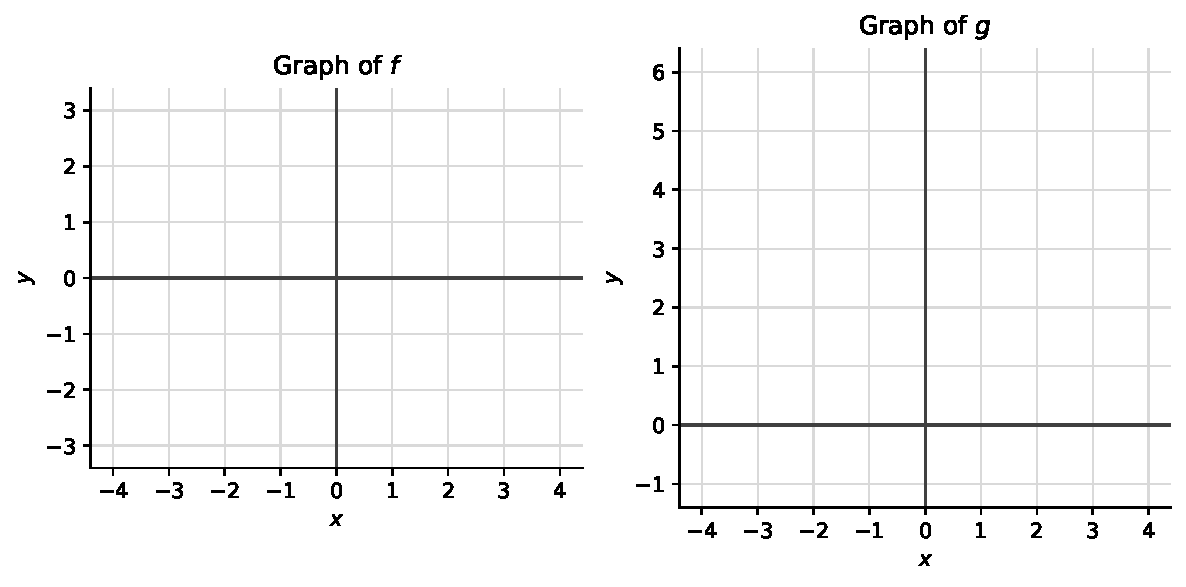
\includegraphics[keepaspectratio]{06_activity_properties_of_functions_files/figure-pdf/fig-blank-axes-output-1.pdf}}

}

\caption{\label{fig-blank-axes}Blank axes for sketching \(f\) (left) and
\(g\) (right).}

\end{figure}%

\section{Step 2: Make an educated
guess}\label{step-2-make-an-educated-guess}

From your graphs, try to answer the following.

\begin{enumerate}
\def\labelenumi{\arabic{enumi}.}
\tightlist
\item
  Is the function injective?
\item
  Is it monotone? If so, is it \emph{strictly} monotone? If not, can you
  find intervals --- as large as possible --- on which it is (strictly)
  monotone?
\item
  Is it even, odd, or neither?
\item
  Is it continuous everywhere? If not, at which \(x\) is it
  discontinuous?
\end{enumerate}

Record short answers in the table; you will verify each one in the steps
that follow.

{\def\LTcaptype{none} % do not increment counter
\begin{longtable}[]{@{}lll@{}}
\toprule\noalign{}
Property & \(f\) & \(g\) \\
\midrule\noalign{}
\endhead
\bottomrule\noalign{}
\endlastfoot
Injective? (yes / no) & ~ & ~ \\
Monotone? Strictly? On which interval(s)? & ~ & ~ \\
Even, odd, or neither? & ~ & ~ \\
Continuous everywhere? If not, at which \(x\)? & ~ & ~ \\
\end{longtable}
}

\section{Verification: injectivity}\label{verification-injectivity}

Neither \(f\) nor \(g\) is injective. To prove this, it is enough to
exhibit two inputs \(x \neq y\) with the same output.

\begin{exercise}[]\protect\hypertarget{exr-activity-injective}{}\label{exr-activity-injective}

Find explicit values:

\begin{itemize}
\tightlist
\item
  for \(f\): \(x = \underline{\qquad}\) and \(y = \underline{\qquad}\)
  with \(f(x) = f(y)\);
\item
  for \(g\): \(x = \underline{\qquad}\) and \(y = \underline{\qquad}\)
  with \(g(x) = g(y)\).
\end{itemize}

\end{exercise}

\section{Verification: even / odd}\label{verification-even-odd}

\begin{exercise}[]\protect\hypertarget{exr-activity-even-odd}{}\label{exr-activity-even-odd}

For whichever symmetry you guessed, verify it directly from the
definition of the function: compute \(f(-x)\) and check that it equals
\(-f(x)\) (odd) or \(f(x)\) (even). Then do the same for \(g\).

\end{exercise}

\section{Verification: monotonicity}\label{verification-monotonicity}

\begin{exercise}[]\protect\hypertarget{exr-activity-monotone}{}\label{exr-activity-monotone}

Verify your monotonicity guess on a suitable interval, directly from the
definition. For instance, to show a function is increasing on an
interval, assume \(x \le y\) in that interval and deduce
\(f(x) \le f(y)\) (use strict inequalities for \emph{strictly}
increasing); argue similarly for decreasing.

\end{exercise}

\section{\texorpdfstring{Continuity: the \(\varepsilon\)--\(\delta\)
game}{Continuity: the \textbackslash varepsilon--\textbackslash delta game}}\label{continuity-the-varepsilondelta-game}

Both \(f\) and \(g\) are continuous at \(x_0 = 1\). Play the
\(\varepsilon\)--\(\delta\) game from Definition~\ref{def-continuity}.

\begin{exercise}[]\protect\hypertarget{exr-activity-eps-delta}{}\label{exr-activity-eps-delta}

~

\begin{enumerate}
\def\labelenumi{\arabic{enumi}.}
\tightlist
\item
  Take \(\varepsilon = 1\). Find a number \(\delta > 0\) such that \[
  \lvert x - 1 \rvert < \delta \quad \Rightarrow \quad\lvert f(x) - f(1) \rvert < 1
  \] (recall \(f(1) = 1\)). Then find such a \(\delta\) for \(g\).
\item
  Repeat with a smaller tolerance, \(\varepsilon = \tfrac{1}{10}\). Does
  the argument really change?
\item
  Can you produce a \(\delta\) that works for an \textbf{arbitrary}
  \(\varepsilon > 0\)?
\end{enumerate}

\end{exercise}

\section{Discontinuities}\label{discontinuities}

Both functions are discontinuous at \(x_0 = 0\). Here it is \emph{you}
who loses the game.

\begin{exercise}[]\protect\hypertarget{exr-activity-discontinuous}{}\label{exr-activity-discontinuous}

Find an \(\varepsilon > 0\) for which \textbf{no} \(\delta\) works ---
that is, however close \(x\) is taken to \(0\), there is always some
such \(x\) with \[
\lvert f(x) - f(0) \rvert \ge \varepsilon.
\] Give such an \(\varepsilon\) for \(f\), and one for \(g\).

\end{exercise}

\part{Limits}

\chapter{Sequences and Convergence}\label{sequences-and-convergence}

\section{Sequences}\label{sequences}

A \textbf{sequence} is an unending list of real numbers \[
a_1,\ a_2,\ a_3,\ \ldots
\] We write \((a_n)_{n\in\mathbb{N}}\), or just \((a_n)\), and call
\(a_n\) the \textbf{\(n\)-th term}. Formally, a sequence is nothing but
a function \[
a\colon \mathbb{N}\to \mathbb{R},
\] where we write \(a_n\) instead of \(a(n)\).

\begin{example}[]\protect\hypertarget{exm-sequences}{}\label{exm-sequences}

\hfill\break
\[
\begin{aligned}
a_n &= \tfrac{1}{n}: & &1,\ \tfrac12,\ \tfrac13,\ \tfrac14,\ \ldots \\[2pt]
b_n &= \tfrac{(-1)^{n+1}}{n}: & &1,\ -\tfrac12,\ \tfrac13,\ -\tfrac14,\ \ldots \\[2pt]
c_n &= \tfrac{n}{n+1}: & &\tfrac12,\ \tfrac23,\ \tfrac34,\ \tfrac45,\ \ldots \\[2pt]
d_n &= \sqrt[n]{p}, \quad p>0 \text{ fixed} \\[2pt]
e_n &= \alpha^n, \quad \alpha>1.
\end{aligned}
\]

\end{example}

\section{The Limit of a Sequence}\label{the-limit-of-a-sequence}

Look at \(a_n = \tfrac1n\). What happens to the terms as \(n\) gets
larger and larger? The values get smaller and smaller, coming
\textbf{arbitrarily close to \(0\)} --- though no term is ever equal to
\(0\). We want to make ``arbitrarily close'' precise.

The idea is to use \(\varepsilon\)-neighborhoods
(Definition~\ref{def-epsilon-neighborhood}): given a tolerance
\(\varepsilon>0\), we ask that \emph{from some point on}, every term of
the sequence lies within \(\varepsilon\) of \(0\).

\begin{definition}[]\protect\hypertarget{def-null-sequence}{}\label{def-null-sequence}

\hfill\break
We say \((a_n)\) \textbf{converges to \(0\)}, written \[
\lim_{n\to\infty} a_n = 0 \qquad\text{or}\qquad a_n \to 0,
\] if for every \(\varepsilon>0\) there exists \(N\in\mathbb{N}\) such
that \[
\lvert a_n \rvert = \lvert a_n - 0 \rvert < \varepsilon\qquad\text{for all } n \ge N.
\]

\end{definition}

The number \(N\) is allowed to depend on \(\varepsilon\) --- a smaller
tolerance will in general require going further out in the sequence. To
emphasize this dependence one sometimes writes \(N(\varepsilon)\).

\begin{example}[]\protect\hypertarget{exm-one-over-n}{}\label{exm-one-over-n}

\hfill\break
\(\lim_{n\to\infty} \tfrac1n = 0\).

\begin{proof}
Let \(\varepsilon>0\). We must find \(N\) so that
\(\tfrac1n < \varepsilon\) for all \(n\ge N\). Now \[
\tfrac1n < \varepsilon\quad \Leftrightarrow \quad\tfrac1\varepsilon< n,
\] so any \(N \in \mathbb{N}\) with \(N > \tfrac1\varepsilon\) works: if
\(n \ge N > \tfrac1\varepsilon\), then \(\tfrac1n < \varepsilon\).

Concretely, for \(\varepsilon= 0.05 = \tfrac{5}{100}\) we need
\(n > \tfrac{100}{5} = 20\), so \(N = 21\) will do.
\end{proof}

\end{example}

\begin{exercise}[]\protect\hypertarget{exr-alternating-null}{}\label{exr-alternating-null}

Show that \(\lim_{n\to\infty} \dfrac{(-1)^{n+1}}{n} = 0\). (Note
\(\lvert b_n \rvert = \tfrac1n\).)

\end{exercise}

\section{Convergence to a General
Limit}\label{convergence-to-a-general-limit}

Now consider \(c_n = \tfrac{n}{n+1}\). The terms get closer and closer
to \(1\), which suggests \(\lim_{n\to\infty} c_n = 1\). The definition
is the same as before, with \(0\) replaced by the candidate limit.

\begin{definition}[]\protect\hypertarget{def-limit}{}\label{def-limit}

\hfill\break
Let \(a\in\mathbb{R}\). We say \((c_n)\) \textbf{converges to \(a\)},
written \(\lim_{n\to\infty} c_n = a\) or \(c_n \to a\), if for every
\(\varepsilon>0\) there exists \(N\in\mathbb{N}\) such that \[
\lvert c_n - a \rvert < \varepsilon\qquad\text{for all } n \ge N.
\] Equivalently: from the \(N\)-th term on, all terms lie in the
\(\varepsilon\)-neighborhood \((a-\varepsilon,\, a+\varepsilon)\). A
sequence is \textbf{convergent} if it converges to some \(a\), and
\textbf{divergent} otherwise.

\end{definition}

\begin{example}[]\protect\hypertarget{exm-n-over-n-plus-1}{}\label{exm-n-over-n-plus-1}

\hfill\break
\(\lim_{n\to\infty} \dfrac{n}{n+1} = 1\). Here \[
\lvert c_n - 1 \rvert = \lvert \frac{n}{n+1} - 1 \rvert = 1 - \frac{n}{n+1} = \frac{1}{n+1}.
\]

Let us check two tolerances. For \(\varepsilon= 1\) we need
\(\tfrac{1}{n+1} < 1\), which holds for every \(n\ge 1\); so \(N = 1\)
works. For \(\varepsilon= \tfrac14\) we need \[
\frac{1}{n+1} < \frac14 \quad \Leftrightarrow \quad 3 < n,
\] so \(N = 4\) works.

In general,
\(\lvert c_n - 1 \rvert = \tfrac{1}{n+1} < \varepsilon\quad \Leftrightarrow \quad n > \tfrac1\varepsilon- 1\),
so any \(N > \tfrac1\varepsilon- 1\) works, and \(c_n \to 1\).

\end{example}

\begin{refremark}
When a limit exists it is \textbf{unique}: if \(c_n \to a\) and
\(c_n \to a'\), then for every \(\varepsilon>0\) we have
\(\lvert a - a' \rvert \le \lvert a - c_n \rvert + \lvert c_n - a' \rvert < 2\varepsilon\)
for large \(n\), so \(\lvert a-a' \rvert = 0\). This is what justifies
speaking of \emph{the} limit and the notation \(\lim_{n\to\infty} c_n\).

\label{rem-limit-unique}

\end{refremark}

\subsection{Divergence}\label{divergence}

To show a sequence \textbf{diverges} we must show it converges to no
limit at all. Negating Definition~\ref{def-limit}: \((c_n)\) does not
converge to \(a\) if there is some \(\varepsilon>0\) such that, no
matter how far out we go, some later term is at least \(\varepsilon\)
away from \(a\).

\begin{example}[]\protect\hypertarget{exm-alternating-diverges}{}\label{exm-alternating-diverges}

\hfill\break
The sequence \(\big((-1)^n\big) = -1, 1, -1, 1, \ldots\) diverges.

\begin{proof}
Suppose \((-1)^n \to a\) for some \(a\). Take \(\varepsilon= 1\). Then
\(\lvert (-1)^n - a \rvert < 1\) for all large \(n\); applying this to
an even and an odd \(n\) gives \(\lvert 1 - a \rvert < 1\) and
\(\lvert -1 - a \rvert < 1\). But then \[
2 = \lvert 1 - (-1) \rvert \le \lvert 1 - a \rvert + \lvert a - (-1) \rvert < 1 + 1 = 2,
\] a contradiction.
\end{proof}

\end{example}

\begin{exercise}[]\protect\hypertarget{exr-sequences-limits}{}\label{exr-sequences-limits}

Investigate the remaining sequences from Example~\ref{exm-sequences}:
\(d_n = \sqrt[n]{p}\) (with \(p>0\) fixed) and \(e_n = \alpha^n\) (with
\(\alpha>1\)). One converges; the other diverges. Which is which, and
what is the limit?

\end{exercise}

\begin{refremark}
For reference: \(\sqrt[n]{p} \to 1\) for every \(p>0\), while
\(\alpha^n\) diverges when \(\alpha>1\) (its terms grow without bound).
Both facts are proved in C\&J §1.6.

\label{rem-sequences-limits-answers}

\end{refremark}

\section{Limit Laws}\label{limit-laws}

Computing \(N(\varepsilon)\) by hand for every sequence quickly becomes
tedious. The following rules let us build limits of complicated
sequences out of simpler ones.

\begin{proposition}[Arithmetic of
limits]\protect\hypertarget{prp-limit-laws}{}\label{prp-limit-laws}

Suppose \(a_n \to a\) and \(b_n \to b\). Then \[
\begin{aligned}
a_n + b_n &\to a + b, & a_n - b_n &\to a - b, \\
a_n \cdot b_n &\to a \cdot b, & \frac{a_n}{b_n} &\to \frac{a}{b} \quad (\text{provided } b \neq 0).
\end{aligned}
\]

\end{proposition}

\begin{example}[]\protect\hypertarget{exm-rational-sequence}{}\label{exm-rational-sequence}

\hfill\break
Find \(\displaystyle\lim_{n\to\infty} \frac{2n^2 - 1}{n^2 + n + 1}\).

Divide numerator and denominator by \(n^2\): \[
\frac{2n^2 - 1}{n^2 + n + 1}
= \frac{2 - \tfrac{1}{n^2}}{1 + \tfrac1n + \tfrac{1}{n^2}}.
\] Now \(\tfrac1n \to 0\) and \(\tfrac{1}{n^2} \to 0\), so by the limit
laws the numerator tends to \(2 - 0 = 2\) and the denominator to
\(1 + 0 + 0 = 1\). Since the denominator limit is nonzero, \[
\lim_{n\to\infty} \frac{2n^2 - 1}{n^2 + n + 1} = \frac{2}{1} = 2.
\]

\end{example}

\section{Comparison and the Squeeze
Theorem}\label{comparison-and-the-squeeze-theorem}

\begin{exercise}[]\protect\hypertarget{exr-warmup-half-n}{}\label{exr-warmup-half-n}

\textbf{Warm-up.} Show that \(\lim_{n\to\infty} \dfrac{1}{2^n} = 0\).

\end{exercise}

Rather than hunting for \(N(\varepsilon)\) from scratch every time, it
is often easier to compare a sequence to one whose limit we already
know.

\begin{proposition}[Comparison
test]\protect\hypertarget{prp-comparison}{}\label{prp-comparison}

Suppose \(0 \le b_n \le a_n\) for all \(n\), and \(a_n \to 0\). Then
\(b_n \to 0\).

\end{proposition}

\begin{proof}
Let \(\varepsilon>0\). Since \(a_n\to0\) there is \(N\in\mathbb{N}\)
with \(a_n < \varepsilon\) for all \(n\ge N\). Then for \(n\ge N\), \[
0 \le b_n \le a_n < \varepsilon,
\] so \(\lvert b_n - 0 \rvert = b_n < \varepsilon\). Hence
\(b_n \to 0\).
\end{proof}

We can generalize this by sandwiching a sequence between two others that
converge to the \emph{same} limit works for any target value.

\begin{proposition}[Squeeze
theorem]\protect\hypertarget{prp-squeeze}{}\label{prp-squeeze}

Suppose \(a_n \le b_n \le c_n\) for all \(n\), and \(a_n \to L\),
\(c_n \to L\) for the same \(L\in\mathbb{R}\). Then \(b_n \to L\).

\end{proposition}

\begin{proof}
Let \(\varepsilon>0\). Choose \(N_1\) with
\(\lvert a_n-L \rvert<\varepsilon\) for \(n\ge N_1\), and \(N_2\) with
\(\lvert c_n-L \rvert<\varepsilon\) for \(n\ge N_2\). Let
\(N=\max(N_1,N_2)\). For \(n\ge N\), \[
L-\varepsilon< a_n \le b_n \le c_n < L+\varepsilon,
\] so \(\lvert b_n-L \rvert<\varepsilon\). Hence \(b_n\to L\).
\end{proof}

\begin{refremark}
Proposition~\ref{prp-comparison} is the special case of the squeeze
theorem where the lower bounding sequence is constantly \(0\) and
\(L=0\).

\label{rem-squeeze-comparison}

\end{refremark}

\section{Monotone and Bounded
Sequences}\label{monotone-and-bounded-sequences}

\begin{definition}[]\protect\hypertarget{def-monotone}{}\label{def-monotone}

\hfill\break
A sequence \((a_n)\) is \textbf{increasing} if \(a_n \le a_{n+1}\) for
all \(n\), and \textbf{decreasing} if \(a_n \ge a_{n+1}\) for all \(n\).
It is \textbf{monotone} if it is increasing or decreasing.

\end{definition}

\begin{definition}[]\protect\hypertarget{def-bounded}{}\label{def-bounded}

\hfill\break
A sequence \((a_n)\) is \textbf{bounded} if there is a constant \(C\)
such that \(\lvert a_n \rvert\le C\) for all \(n\).

\end{definition}

\begin{theorem}[Monotone Convergence
Theorem]\protect\hypertarget{thm-monotone-convergence}{}\label{thm-monotone-convergence}

Every bounded monotone sequence converges.

\end{theorem}

\begin{refremark}
This theorem expresses the same completeness of \(\mathbb{R}\) as the
Nested Interval Axiom from \hyperref[the-nested-interval-axiom]{The
Nested Interval Axiom} --- each can be derived from the other. We will
not reprove the general statement here; instead we isolate the paired
form that we actually use below, which follows directly from the axiom
together with the comparison test.

\label{rem-monotone-nip}

\end{refremark}

\begin{corollary}[]\protect\hypertarget{cor-monotone-squeeze}{}\label{cor-monotone-squeeze}

Suppose \((a_n)\) is increasing, \((b_n)\) is decreasing, \(a_n\le b_n\)
for all \(n\), and \(b_n - a_n \to 0\). Then \((a_n)\) and \((b_n)\)
converge to a common limit \(c\), the unique point in
\(\bigcap_n [a_n,b_n]\).

\end{corollary}

\begin{proof}
Since \((a_n)\) is increasing and \((b_n)\) is decreasing with
\(a_n\le b_n\), the intervals \([a_n,b_n]\) are nested:
\([a_{n+1},b_{n+1}]\subseteq[a_n,b_n]\) for all \(n\). By the Nested
Interval Axiom there is a point \(c\) with \(a_n \le c \le b_n\) for
every \(n\). Then \[
0 \le c - a_n \le b_n - a_n \to 0 \qquad\text{and}\qquad 0 \le b_n - c \le b_n - a_n \to 0,
\] so the comparison test (Proposition~\ref{prp-comparison}) gives
\(a_n \to c\) and \(b_n \to c\).
\end{proof}

\section{Applications}\label{applications}

\begin{lemma}[Bernoulli's
inequality]\protect\hypertarget{lem-bernoulli}{}\label{lem-bernoulli}

For \(c \ge -1\) and \(n\in\mathbb{N}\), \[
(1+c)^n \ge 1 + nc.
\]

\end{lemma}

(For \(c \geq 0\) one can prove this by considering just the first two
terms of the
\href{https://en.wikipedia.org/wiki/Binomial_theorem}{binomial
expansion} of \((1+c)^n\). The remaining terms are all non-negative, so
by leaving them out, we obtain something smaller.)

\subsection{\texorpdfstring{Roots:
\(\sqrt[n]{p} \to 1\)}{Roots: \textbackslash sqrt{[}n{]}\{p\} \textbackslash to 1}}\label{roots-sqrtnp-to-1}

\begin{theorem}[]\protect\hypertarget{thm-nth-root}{}\label{thm-nth-root}

\hfill\break
For every \(p>0\), \(\displaystyle\lim_{n\to\infty}\sqrt[n]{p} = 1\).

\end{theorem}

\begin{proof}
For \(p=1\) the sequence is constant, so there is nothing to show.

Suppose \(p>1\). Write \(a_n := \sqrt[n]{p} = 1+\delta_n\); since
\(p>1\) we have \(a_n>1\), so \(\delta_n>0\). Raising to the \(n\)-th
power and applying Bernoulli's inequality (with \(c=\delta_n\ge0\)), \[
p = (1+\delta_n)^n \ge 1+n\delta_n,
\] so \(0 < \delta_n \le \dfrac{p-1}{n}\). Since \(\tfrac{p-1}{n}\to0\),
the comparison test gives \(\delta_n\to0\), and hence
\(a_n = 1+\delta_n \to 1\).

Suppose \(0<p<1\). Then \(q:=1/p>1\), and by the case just proved
\(\sqrt[n]{q}\to1\). Since \(\sqrt[n]{q}\neq0\) for all \(n\) and its
limit is nonzero, the quotient rule in Proposition~\ref{prp-limit-laws}
gives \[
\sqrt[n]{p} = \frac{1}{\sqrt[n]{q}} \longrightarrow \frac11 = 1.
\]
\end{proof}

This proves the claim recorded in
Remark~\ref{rem-sequences-limits-answers} for \(d_n=\sqrt[n]{p}\).

\subsection{\texorpdfstring{The Number
\(e\)}{The Number e}}\label{the-number-e}

\begin{proposition}[]\protect\hypertarget{prp-e-increasing}{}\label{prp-e-increasing}

\hfill\break
The sequence \(e_n := \left(1+\tfrac1n\right)^n\) is increasing.

\end{proposition}

\begin{proof}
We must show \[
\left(1+\frac1n\right)^n \le \left(1+\frac1{n+1}\right)^{n+1}. \tag{$*$}
\] Writing both sides with a common fractional base and splitting off
one factor of \(\tfrac{n+2}{n+1}\) on the right, \[
(*) \iff \left(\frac{n+1}{n}\right)^n \le \left(\frac{n+2}{n+1}\right)^n \cdot \frac{n+2}{n+1}
\iff \frac{n+1}{n+2} \le \left(\frac{n(n+2)}{(n+1)^2}\right)^{n}.
\] Since \((n+1)^2 = n^2+2n+1\), we have
\(n(n+2) = n^2+2n = (n+1)^2-1\), so \[
\left(\frac{n(n+2)}{(n+1)^2}\right)^{n} = \left(1-\frac{1}{(n+1)^2}\right)^{n}.
\] By Bernoulli's inequality (with \(c=-\tfrac{1}{(n+1)^2}\ge-1\)), \[
\left(1-\frac{1}{(n+1)^2}\right)^{n} \ge 1 - \frac{n}{(n+1)^2}.
\] So it suffices to show \(\dfrac{n+1}{n+2} \le 1-\dfrac{n}{(n+1)^2}\),
i.e. \[
\frac{1}{n+2} \ge \frac{n}{(n+1)^2} \iff (n+1)^2 \ge n(n+2) \iff n^2+2n+1 \ge n^2+2n,
\] which is always true. Chaining the inequalities back together proves
\((*)\).
\end{proof}

\begin{exercise}[]\protect\hypertarget{exr-f-decreasing}{}\label{exr-f-decreasing}

Show that \(f_n := \left(1+\tfrac1n\right)^{n+1}\) is decreasing. (Adapt
the computation in the proof of Proposition~\ref{prp-e-increasing}.)

\end{exercise}

\begin{theorem}[]\protect\hypertarget{thm-e-exists}{}\label{thm-e-exists}

\hfill\break
The limit \[
e := \lim_{n\to\infty}\left(1+\frac1n\right)^n
\] exists; numerically \(e \approx 2.71828\ldots\).

\end{theorem}

\begin{proof}
Let \(e_n = \left(1+\tfrac1n\right)^n\) and
\(f_n = \left(1+\tfrac1n\right)^{n+1} = e_n\left(1+\tfrac1n\right)\), so
\(e_n \le f_n\) for all \(n\). By Proposition~\ref{prp-e-increasing},
\((e_n)\) is increasing; by Exercise~\ref{exr-f-decreasing}, \((f_n)\)
is decreasing. In particular \(e_n \le f_n \le f_1 = 4\) for all \(n\),
so \((e_n)\) is bounded.

Moreover \[
0 \le f_n - e_n = e_n\cdot\frac1n \le \frac{f_1}{n} = \frac4n \longrightarrow 0,
\] so \(f_n - e_n \to 0\) by the comparison test. By
Corollary~\ref{cor-monotone-squeeze}, \((e_n)\) and \((f_n)\) converge
to a common limit --- which we call \(e\). Numerically,
\(e_{10} \approx 2.594\), \(e_{100}\approx 2.705\),
\(e_{1000}\approx 2.7169\), consistent with \(e\approx 2.71828\ldots\).
\end{proof}

\section{Summary}\label{summary-5}

\begin{itemize}
\tightlist
\item
  A \textbf{sequence} is a function \(a\colon\mathbb{N}\to\mathbb{R}\),
  written \((a_n)\).
\item
  \((a_n)\) \textbf{converges to \(a\)} (Definition~\ref{def-limit}) if
  for every tolerance \(\varepsilon>0\) there is an index \(N\) such
  that \(\lvert a_n - a \rvert < \varepsilon\) for all \(n\ge N\) ---
  from some point on, all terms lie in the \(\varepsilon\)-neighborhood
  of \(a\). The special case \(a=0\) is
  Definition~\ref{def-null-sequence}.
\item
  The limit, when it exists, is \textbf{unique}
  (Remark~\ref{rem-limit-unique}). A sequence with no limit, such as
  \(\big((-1)^n\big)\) (Example~\ref{exm-alternating-diverges}), is
  \textbf{divergent}.
\item
  The \textbf{limit laws} (Proposition~\ref{prp-limit-laws}) compute
  limits of sums, differences, products, and quotients termwise;
  dividing through by the highest power of \(n\) turns a ratio of
  polynomials into a form where they apply
  (Example~\ref{exm-rational-sequence}).
\item
  The \textbf{comparison test} and \textbf{squeeze theorem}
  (Proposition~\ref{prp-comparison}, Proposition~\ref{prp-squeeze}) let
  us find a limit by trapping a sequence between two others whose limits
  we already know.
\item
  A \textbf{bounded monotone sequence converges}
  (Theorem~\ref{thm-monotone-convergence}), a fact equivalent to the
  Nested Interval Axiom; the paired form
  (Corollary~\ref{cor-monotone-squeeze}) --- an increasing and a
  decreasing sequence squeezing together --- is the version we use in
  practice.
\item
  \textbf{Bernoulli's inequality} \((1+c)^n \ge 1+nc\)
  (Lemma~\ref{lem-bernoulli}) drives two applications: every
  \(\sqrt[n]{p} \to 1\) (Theorem~\ref{thm-nth-root}), and
  \(\left(1+\tfrac1n\right)^n\) increases while
  \(\left(1+\tfrac1n\right)^{n+1}\) decreases to the same limit,
  defining the number \(e\approx2.71828\ldots\)
  (Theorem~\ref{thm-e-exists}).
\end{itemize}

\chapter{Convergence of Sequences: Reading
Data}\label{convergence-of-sequences-reading-data}

\begin{Shaded}
\begin{Highlighting}[]
\CommentTok{\#}
\CommentTok{\# !!! RUN THIS FIRST !!!}
\CommentTok{\#}
\CommentTok{\# (loads the data and defines all necessary functions)}
\CommentTok{\#}


\ImportTok{import}\NormalTok{ numpy }\ImportTok{as}\NormalTok{ np}
\ImportTok{import}\NormalTok{ pandas }\ImportTok{as}\NormalTok{ pd}
\ImportTok{import}\NormalTok{ matplotlib.pyplot }\ImportTok{as}\NormalTok{ plt}

\NormalTok{pd.set\_option(}\StringTok{\textquotesingle{}display.max\_rows\textquotesingle{}}\NormalTok{, }\DecValTok{20}\NormalTok{)  }\CommentTok{\# long tables show head/tail with \textquotesingle{}...\textquotesingle{} automatically}

\NormalTok{df }\OperatorTok{=}\NormalTok{ pd.read\_csv(}\StringTok{\textquotesingle{}data/rc\_circuit\_data.csv\textquotesingle{}}\NormalTok{)}

\KeywordTok{def}\NormalTok{ a(n):}
    \CommentTok{"""Return the n{-}th term of the sequence, a\_n, as a plain float."""}
\NormalTok{    row }\OperatorTok{=}\NormalTok{ df.loc[df[}\StringTok{\textquotesingle{}n\textquotesingle{}}\NormalTok{] }\OperatorTok{==}\NormalTok{ n]}
    \ControlFlowTok{if}\NormalTok{ row.empty:}
        \ControlFlowTok{raise} \PreprocessorTok{ValueError}\NormalTok{(}\SpecialStringTok{f"n = }\SpecialCharTok{\{}\NormalTok{n}\SpecialCharTok{\}}\SpecialStringTok{ is out of range (data covers n = 0 .. }\SpecialCharTok{\{}\NormalTok{df[}\StringTok{\textquotesingle{}n\textquotesingle{}}\NormalTok{]}\SpecialCharTok{.}\BuiltInTok{max}\NormalTok{()}\SpecialCharTok{\}}\SpecialStringTok{)."}\NormalTok{)}
    \ControlFlowTok{return} \BuiltInTok{float}\NormalTok{(row[}\StringTok{\textquotesingle{}measured\_value\textquotesingle{}}\NormalTok{].values[}\DecValTok{0}\NormalTok{])}

\KeywordTok{def}\NormalTok{ find\_smallest\_N(data, L\_guess, epsilon, value\_col}\OperatorTok{=}\StringTok{\textquotesingle{}measured\_value\textquotesingle{}}\NormalTok{):}
    \CommentTok{"""Smallest N (present in the data) such that all later points are within epsilon of L\_guess."""}
\NormalTok{    vals }\OperatorTok{=}\NormalTok{ data[value\_col].values}
\NormalTok{    n\_vals }\OperatorTok{=}\NormalTok{ data[}\StringTok{\textquotesingle{}n\textquotesingle{}}\NormalTok{].values}
    \ControlFlowTok{for}\NormalTok{ i }\KeywordTok{in} \BuiltInTok{range}\NormalTok{(}\BuiltInTok{len}\NormalTok{(vals)):}
        \ControlFlowTok{if}\NormalTok{ np.}\BuiltInTok{all}\NormalTok{(np.}\BuiltInTok{abs}\NormalTok{(vals[i:] }\OperatorTok{{-}}\NormalTok{ L\_guess) }\OperatorTok{\textless{}}\NormalTok{ epsilon):}
            \ControlFlowTok{return} \BuiltInTok{int}\NormalTok{(n\_vals[i])}
    \ControlFlowTok{return} \VariableTok{None}


\KeywordTok{def}\NormalTok{ check\_convergence(data, L\_guess, N\_guess, epsilon, value\_col}\OperatorTok{=}\StringTok{\textquotesingle{}measured\_value\textquotesingle{}}\NormalTok{, reveal\_threshold}\OperatorTok{=}\DecValTok{50}\NormalTok{):}
\NormalTok{    vals }\OperatorTok{=}\NormalTok{ data[value\_col].values}
\NormalTok{    n\_vals }\OperatorTok{=}\NormalTok{ data[}\StringTok{\textquotesingle{}n\textquotesingle{}}\NormalTok{].values}
\NormalTok{    mask }\OperatorTok{=}\NormalTok{ n\_vals }\OperatorTok{\textgreater{}=}\NormalTok{ N\_guess}

    \ControlFlowTok{if} \KeywordTok{not}\NormalTok{ mask.}\BuiltInTok{any}\NormalTok{():}
        \BuiltInTok{print}\NormalTok{(}\SpecialStringTok{f"N\_guess = }\SpecialCharTok{\{}\NormalTok{N\_guess}\SpecialCharTok{\}}\SpecialStringTok{ is beyond the range of available data (max n = }\SpecialCharTok{\{}\NormalTok{n\_vals}\SpecialCharTok{.}\BuiltInTok{max}\NormalTok{()}\SpecialCharTok{\}}\SpecialStringTok{)."}\NormalTok{)}
        \ControlFlowTok{return} \VariableTok{False}

\NormalTok{    tail\_n }\OperatorTok{=}\NormalTok{ n\_vals[mask]}
\NormalTok{    tail\_vals }\OperatorTok{=}\NormalTok{ vals[mask]}
\NormalTok{    bad }\OperatorTok{=}\NormalTok{ np.}\BuiltInTok{abs}\NormalTok{(tail\_vals }\OperatorTok{{-}}\NormalTok{ L\_guess) }\OperatorTok{\textgreater{}=}\NormalTok{ epsilon}

    \ControlFlowTok{if}\NormalTok{ bad.}\BuiltInTok{any}\NormalTok{():}
\NormalTok{        first\_bad\_n }\OperatorTok{=}\NormalTok{ tail\_n[bad][}\DecValTok{0}\NormalTok{]}
        \BuiltInTok{print}\NormalTok{(}\SpecialStringTok{f"✗ Not valid: at n = }\SpecialCharTok{\{}\NormalTok{first\_bad\_n}\SpecialCharTok{\}}\SpecialStringTok{, |a\_n {-} }\SpecialCharTok{\{}\NormalTok{L\_guess}\SpecialCharTok{\}}\SpecialStringTok{| \textgreater{}= }\SpecialCharTok{\{}\NormalTok{epsilon}\SpecialCharTok{\}}\SpecialStringTok{."}\NormalTok{)}
        \BuiltInTok{print}\NormalTok{(}\StringTok{"  The sequence leaves the epsilon{-}band after your N\_guess. Try a larger N, "}
              \StringTok{"or reconsider your L\_guess."}\NormalTok{)}
        \ControlFlowTok{return} \VariableTok{False}

    \BuiltInTok{print}\NormalTok{(}\SpecialStringTok{f"✓ Valid: for all n \textgreater{}= }\SpecialCharTok{\{}\NormalTok{N\_guess}\SpecialCharTok{\}}\SpecialStringTok{, |a\_n {-} }\SpecialCharTok{\{}\NormalTok{L\_guess}\SpecialCharTok{\}}\SpecialStringTok{| \textless{} }\SpecialCharTok{\{}\NormalTok{epsilon}\SpecialCharTok{\}}\SpecialStringTok{."}\NormalTok{)}

    \CommentTok{\# Don\textquotesingle{}t just hand over the smallest N {-}{-} only reveal it once the guess is close.}
\NormalTok{    best\_N }\OperatorTok{=}\NormalTok{ find\_smallest\_N(data, L\_guess, epsilon, value\_col)}
    \ControlFlowTok{if}\NormalTok{ best\_N }\KeywordTok{is} \KeywordTok{not} \VariableTok{None}\NormalTok{:}
\NormalTok{        gap }\OperatorTok{=}\NormalTok{ N\_guess }\OperatorTok{{-}}\NormalTok{ best\_N}
        \ControlFlowTok{if}\NormalTok{ gap }\OperatorTok{==} \DecValTok{0}\NormalTok{:}
            \BuiltInTok{print}\NormalTok{(}\StringTok{"  This is also the smallest N that works for this L\_guess."}\NormalTok{)}
        \ControlFlowTok{elif}\NormalTok{ gap }\OperatorTok{\textless{}=}\NormalTok{ reveal\_threshold:}
            \BuiltInTok{print}\NormalTok{(}\SpecialStringTok{f"  Close! The smallest N that works is N = }\SpecialCharTok{\{}\NormalTok{best\_N}\SpecialCharTok{\}}\SpecialStringTok{ (you were only }\SpecialCharTok{\{}\NormalTok{gap}\SpecialCharTok{\}}\SpecialStringTok{ away)."}\NormalTok{)}
        \ControlFlowTok{else}\NormalTok{:}
            \BuiltInTok{print}\NormalTok{(}\StringTok{"  This N works, but it\textquotesingle{}s probably not the smallest one {-}{-} "}
                  \StringTok{"try a smaller N and see if it still holds."}\NormalTok{)}
    \ControlFlowTok{return} \VariableTok{True}


\KeywordTok{def}\NormalTok{ plot\_challenge(data, L\_guess, N\_guess}\OperatorTok{=}\VariableTok{None}\NormalTok{, epsilon}\OperatorTok{=}\VariableTok{None}\NormalTok{, value\_col}\OperatorTok{=}\StringTok{\textquotesingle{}measured\_value\textquotesingle{}}\NormalTok{,}
\NormalTok{                    zoom}\OperatorTok{=}\VariableTok{True}\NormalTok{, }\BuiltInTok{buffer}\OperatorTok{=}\DecValTok{50}\NormalTok{):}
    \CommentTok{"""}
\CommentTok{    Plot the sequence with the guessed L (and epsilon band, and N\_guess) marked.}

\CommentTok{    By default (zoom=True), the plot starts \textasciigrave{}buffer\textasciigrave{} samples before N\_guess and}
\CommentTok{    runs to the end of the data {-}{-} enough to see whether the sequence was}
\CommentTok{    outside the band right before N\_guess, and to see it stay inside the band}
\CommentTok{    all the way to the end. Set zoom=False to see the whole sequence instead,}
\CommentTok{    or pass a bigger \textasciigrave{}buffer\textasciigrave{} to look further back.}
\CommentTok{    """}
\NormalTok{    plot\_data }\OperatorTok{=}\NormalTok{ data}
    \ControlFlowTok{if}\NormalTok{ zoom }\KeywordTok{and}\NormalTok{ N\_guess }\KeywordTok{is} \KeywordTok{not} \VariableTok{None}\NormalTok{:}
\NormalTok{        start }\OperatorTok{=} \BuiltInTok{max}\NormalTok{(}\BuiltInTok{int}\NormalTok{(data[}\StringTok{\textquotesingle{}n\textquotesingle{}}\NormalTok{].}\BuiltInTok{min}\NormalTok{()), N\_guess }\OperatorTok{{-}} \BuiltInTok{buffer}\NormalTok{)}
\NormalTok{        mask }\OperatorTok{=}\NormalTok{ data[}\StringTok{\textquotesingle{}n\textquotesingle{}}\NormalTok{] }\OperatorTok{\textgreater{}=}\NormalTok{ start}
\NormalTok{        plot\_data }\OperatorTok{=}\NormalTok{ data[mask]}

\NormalTok{    plt.figure(figsize}\OperatorTok{=}\NormalTok{(}\DecValTok{8}\NormalTok{, }\DecValTok{4}\NormalTok{))}
\NormalTok{    plt.plot(plot\_data[}\StringTok{\textquotesingle{}n\textquotesingle{}}\NormalTok{], plot\_data[value\_col], }\StringTok{\textquotesingle{}.\textquotesingle{}}\NormalTok{, alpha}\OperatorTok{=}\FloatTok{0.6}\NormalTok{)}
\NormalTok{    plt.axhline(L\_guess, color}\OperatorTok{=}\StringTok{\textquotesingle{}green\textquotesingle{}}\NormalTok{, linestyle}\OperatorTok{=}\StringTok{\textquotesingle{}{-}{-}\textquotesingle{}}\NormalTok{, label}\OperatorTok{=}\SpecialStringTok{f\textquotesingle{}L\_guess = }\SpecialCharTok{\{}\NormalTok{L\_guess}\SpecialCharTok{\}}\SpecialStringTok{\textquotesingle{}}\NormalTok{)}
    \ControlFlowTok{if}\NormalTok{ epsilon }\KeywordTok{is} \KeywordTok{not} \VariableTok{None}\NormalTok{:}
\NormalTok{        plt.fill\_between(plot\_data[}\StringTok{\textquotesingle{}n\textquotesingle{}}\NormalTok{], L\_guess }\OperatorTok{{-}}\NormalTok{ epsilon, L\_guess }\OperatorTok{+}\NormalTok{ epsilon,}
\NormalTok{                          color}\OperatorTok{=}\StringTok{\textquotesingle{}green\textquotesingle{}}\NormalTok{, alpha}\OperatorTok{=}\FloatTok{0.15}\NormalTok{, label}\OperatorTok{=}\SpecialStringTok{f\textquotesingle{}epsilon band (+/{-} }\SpecialCharTok{\{}\NormalTok{epsilon}\SpecialCharTok{\}}\SpecialStringTok{)\textquotesingle{}}\NormalTok{)}
    \ControlFlowTok{if}\NormalTok{ N\_guess }\KeywordTok{is} \KeywordTok{not} \VariableTok{None}\NormalTok{:}
\NormalTok{        plt.axvline(N\_guess, color}\OperatorTok{=}\StringTok{\textquotesingle{}red\textquotesingle{}}\NormalTok{, linestyle}\OperatorTok{=}\StringTok{\textquotesingle{}:\textquotesingle{}}\NormalTok{, label}\OperatorTok{=}\SpecialStringTok{f\textquotesingle{}N\_guess = }\SpecialCharTok{\{}\NormalTok{N\_guess}\SpecialCharTok{\}}\SpecialStringTok{\textquotesingle{}}\NormalTok{)}
\NormalTok{    plt.xlabel(}\StringTok{\textquotesingle{}n\textquotesingle{}}\NormalTok{)}
\NormalTok{    plt.ylabel(value\_col)}
\NormalTok{    plt.legend()}
\NormalTok{    plt.show()}
\end{Highlighting}
\end{Shaded}

You've been handed a log file, \texttt{data/rc\_circuit\_data.csv}, from
a lab sensor. It records a voltage measurement \texttt{measured\_value}
at each sample index \texttt{n} (and the corresponding time
\texttt{t\_seconds}).

\textbf{You do not know what circuit or process produced this data.}
Your job is to:

\begin{enumerate}
\def\labelenumi{\arabic{enumi}.}
\tightlist
\item
  Explore the data and form a hypothesis about its limiting behavior.
\item
  Given a challenge value \(\varepsilon\), \textbf{guess} the limit
  \(L\) and the index \(N\) after which the data stays within
  \(\varepsilon\) of \(L\) --- then verify your guess rigorously, not
  just by eye.
\end{enumerate}

Recall the definition:

\[ \lim_{n\to\infty} a_n = L \iff \text{ for all } \varepsilon>0,\ \text{ there is } N \text{ s.t. } n\ge N \implies |a_n-L|<\varepsilon. \]

\section{A Simple Query Function}\label{a-simple-query-function}

Sometimes you just want a single term of the sequence, \(a_n\), without
pulling up the whole table. \texttt{a(n)} does that.

\begin{Shaded}
\begin{Highlighting}[]
\CommentTok{\# try it:}

\NormalTok{a(}\DecValTok{0}\NormalTok{), a(}\DecValTok{5000}\NormalTok{), a(}\DecValTok{9999}\NormalTok{)}
\end{Highlighting}
\end{Shaded}

\begin{verbatim}
(0.0, 5.0165, 4.9733)
\end{verbatim}

\section{Task 1: Explore the Data}\label{task-1-explore-the-data}

The full log has 10,000 samples. Set \texttt{n\_start} and
\texttt{n\_end} below to pick a window and re-run the cell to see the
table and plot over just that range --- e.g.~zoom into the early samples
to see the initial behavior, or into the tail to see whether it's still
moving. Change the numbers and re-run as many times as you like.

\begin{Shaded}
\begin{Highlighting}[]
\CommentTok{\# EDIT HERE}

\NormalTok{n\_start }\OperatorTok{=} \DecValTok{3000}
\NormalTok{n\_end }\OperatorTok{=} \DecValTok{9000}


\CommentTok{\#}
\CommentTok{\# No need to change anything down here}
\CommentTok{\#}
\NormalTok{view }\OperatorTok{=}\NormalTok{ df[(df[}\StringTok{\textquotesingle{}n\textquotesingle{}}\NormalTok{] }\OperatorTok{\textgreater{}=}\NormalTok{ n\_start) }\OperatorTok{\&}\NormalTok{ (df[}\StringTok{\textquotesingle{}n\textquotesingle{}}\NormalTok{] }\OperatorTok{\textless{}=}\NormalTok{ n\_end)]}
\NormalTok{display(view)}

\NormalTok{plt.figure(figsize}\OperatorTok{=}\NormalTok{(}\DecValTok{8}\NormalTok{, }\DecValTok{4}\NormalTok{))}
\NormalTok{plt.plot(view[}\StringTok{\textquotesingle{}n\textquotesingle{}}\NormalTok{], view[}\StringTok{\textquotesingle{}measured\_value\textquotesingle{}}\NormalTok{], }\StringTok{\textquotesingle{}.\textquotesingle{}}\NormalTok{, alpha}\OperatorTok{=}\FloatTok{0.7}\NormalTok{)}
\NormalTok{plt.xlabel(}\StringTok{\textquotesingle{}n\textquotesingle{}}\NormalTok{)}
\NormalTok{plt.ylabel(}\StringTok{\textquotesingle{}measured\_value\textquotesingle{}}\NormalTok{)}
\NormalTok{plt.title(}\SpecialStringTok{f\textquotesingle{}Sensor log, n = }\SpecialCharTok{\{}\NormalTok{n\_start}\SpecialCharTok{\}}\SpecialStringTok{ to }\SpecialCharTok{\{}\NormalTok{n\_end}\SpecialCharTok{\}}\SpecialStringTok{\textquotesingle{}}\NormalTok{)}
\NormalTok{plt.show()}
\end{Highlighting}
\end{Shaded}

{\def\LTcaptype{none} % do not increment counter
\begin{longtable}[]{@{}llll@{}}
\toprule\noalign{}
& n & t\_seconds & measured\_value \\
\midrule\noalign{}
\endhead
\bottomrule\noalign{}
\endlastfoot
3000 & 3000 & 0.3000 & 4.9917 \\
3001 & 3001 & 0.3001 & 4.9966 \\
3002 & 3002 & 0.3002 & 4.9946 \\
3003 & 3003 & 0.3003 & 4.9709 \\
3004 & 3004 & 0.3004 & 5.0027 \\
... & ... & ... & ... \\
8996 & 8996 & 0.8996 & 5.0257 \\
8997 & 8997 & 0.8997 & 4.9995 \\
8998 & 8998 & 0.8998 & 4.9907 \\
8999 & 8999 & 0.8999 & 4.9952 \\
9000 & 9000 & 0.9000 & 5.0096 \\
\end{longtable}
}

\pandocbounded{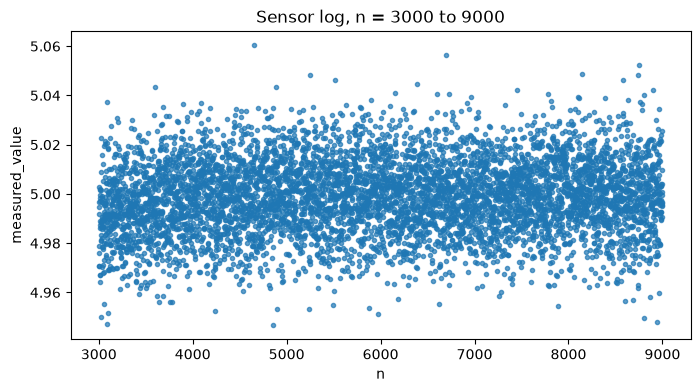
\includegraphics[keepaspectratio]{notebooks/Week03_convergence_files/figure-pdf/cell-4-output-2.png}}

\subsection{Questions to answer before moving
on}\label{questions-to-answer-before-moving-on}

\begin{itemize}
\tightlist
\item
  What value does the sequence appear to be approaching? Write down your
  best guess for \(L\).
\item
  Roughly how many samples does it take before the data ``settles down''
  near that value?
\item
  Does the data ever exceed your guessed \(L\), or only approach it from
  below?
\item
  Try \texttt{a(n)} for a few large \texttt{n} (e.g.~7000, 8500, 9999)
  --- does it match what the plot suggested?
\end{itemize}

\section{\texorpdfstring{Task 2: The \(\varepsilon\)
Challenge}{Task 2: The \textbackslash varepsilon Challenge}}\label{task-2-the-varepsilon-challenge}

Your instructor assigns a value of \(\varepsilon\). Using \textbf{only
the data} (no formulas, no ground truth), you must:

\begin{enumerate}
\def\labelenumi{\arabic{enumi}.}
\tightlist
\item
  State your guessed limit \texttt{L\_guess}.
\item
  State the smallest index \texttt{N\_guess} you believe works.
\item
  Check your answer with \texttt{check\_convergence} below, which
  verifies directly against the definition: it checks whether
  \textbf{every} remaining data point from \texttt{N\_guess} onward is
  within \texttt{epsilon} of your \texttt{L\_guess}.
\end{enumerate}

Note this checks self-consistency with your own guessed \(L\) --- it
does not tell you the ``true'' limit, because the whole point is that
you don't get to see that. Two different reasonable guesses for \(L\)
can each have a valid \(N\).

The checker also won't just hand you the smallest possible \(N\): if
your guess is close (within 50), it'll tell you the exact smallest
\(N\); if you're further off, it'll just tell you to try smaller.

\texttt{plot\_challenge} zooms in by default: it starts a bit before
your \texttt{N\_guess} and runs to the end of the data, so you can see
both whether the sequence was outside the band just before
\texttt{N\_guess} and that it stays inside all the way to the end. Pass
\texttt{zoom=False} if you want to see the whole sequence instead.

\begin{Shaded}
\begin{Highlighting}[]
\CommentTok{\# {-}{-}{-} Your answer {-}{-}{-}}
\NormalTok{EPSILON }\OperatorTok{=} \FloatTok{0.08}          \CommentTok{\# \textless{}{-} instructor{-}assigned challenge value}

\NormalTok{L\_guess }\OperatorTok{=} \DecValTok{5}         \CommentTok{\# }\AlertTok{TODO}\CommentTok{: your guessed limit}
\NormalTok{N\_guess }\OperatorTok{=} \DecValTok{2400}           \CommentTok{\# }\AlertTok{TODO}\CommentTok{: your guessed N}

\NormalTok{check\_convergence(df, L\_guess, N\_guess, EPSILON)}
\NormalTok{plot\_challenge(df, L\_guess, N\_guess, EPSILON)}
\end{Highlighting}
\end{Shaded}

\begin{verbatim}
✓ Valid: for all n >= 2400, |a_n - 5| < 0.08.
  Close! The smallest N that works is N = 2361 (you were only 39 away).
\end{verbatim}

\pandocbounded{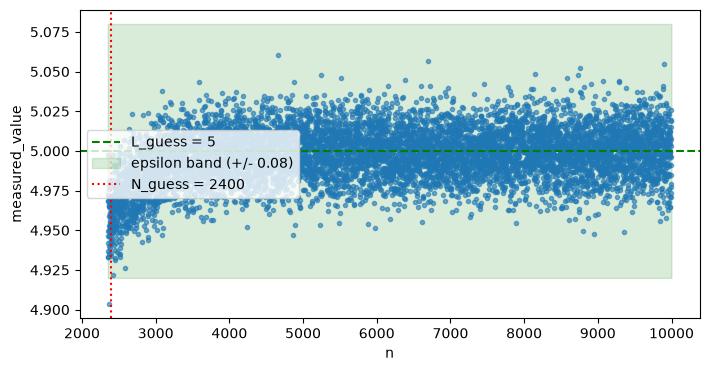
\includegraphics[keepaspectratio]{notebooks/Week03_convergence_files/figure-pdf/cell-5-output-2.png}}

\section{Dataset 2: Damped
Oscillator}\label{dataset-2-damped-oscillator}

This time there's no CSV and no noise. Instead, you're given the
sequence directly as a \textbf{function} you can call for any index
\texttt{n} --- exactly the way a sequence \((b_n)\) is usually presented
in a calculus course. It models the position of an underdamped
mechanical system (e.g.~a suspension, a sensor needle) responding to a
step input:

\[ b_n = x_{ss}\left(1 - e^{-\zeta \omega_n t_n}\left(\cos(\omega_d t_n) +
\frac{\zeta}{\sqrt{1-\zeta^2}}\sin(\omega_d t_n)\right)\right), \qquad t_n = n \cdot dt \]

with \(\omega_d = \omega_n\sqrt{1-\zeta^2}\). Unlike Dataset 1, this
sequence \textbf{oscillates} around its limit before settling --- so
``getting close once'' is not enough; you have to check it \emph{stays}
close.

Since it's an exact formula (not a fixed table), you can evaluate it at
\emph{any} \texttt{n} you like, no matter how large --- there's no upper
limit like there was with \texttt{a(n)}.

\begin{Shaded}
\begin{Highlighting}[]
\NormalTok{x\_ss }\OperatorTok{=} \FloatTok{2.0}     \CommentTok{\# steady{-}state value}
\NormalTok{zeta }\OperatorTok{=} \FloatTok{0.1}     \CommentTok{\# damping ratio}
\NormalTok{wn }\OperatorTok{=} \FloatTok{10.0}      \CommentTok{\# natural frequency (rad/s)}
\NormalTok{wd }\OperatorTok{=}\NormalTok{ wn }\OperatorTok{*}\NormalTok{ np.sqrt(}\DecValTok{1} \OperatorTok{{-}}\NormalTok{ zeta}\OperatorTok{**}\DecValTok{2}\NormalTok{)}
\NormalTok{dt2 }\OperatorTok{=} \FloatTok{0.001}    \CommentTok{\# seconds per sample}

\KeywordTok{def}\NormalTok{ b(n):}
    \CommentTok{"""Return the n{-}th term of the damped step{-}response sequence, b\_n, as a}
\CommentTok{    plain float (or array of floats if n is array{-}like). No noise: this is}
\CommentTok{    the exact closed{-}form value."""}
\NormalTok{    scalar\_input }\OperatorTok{=}\NormalTok{ np.ndim(n) }\OperatorTok{==} \DecValTok{0}
\NormalTok{    t }\OperatorTok{=}\NormalTok{ np.atleast\_1d(np.asarray(n, dtype}\OperatorTok{=}\BuiltInTok{float}\NormalTok{)) }\OperatorTok{*}\NormalTok{ dt2}
\NormalTok{    vals }\OperatorTok{=}\NormalTok{ x\_ss }\OperatorTok{*}\NormalTok{ (}\DecValTok{1} \OperatorTok{{-}}\NormalTok{ np.exp(}\OperatorTok{{-}}\NormalTok{zeta }\OperatorTok{*}\NormalTok{ wn }\OperatorTok{*}\NormalTok{ t) }\OperatorTok{*}
\NormalTok{                    (np.cos(wd }\OperatorTok{*}\NormalTok{ t) }\OperatorTok{+}\NormalTok{ (zeta }\OperatorTok{/}\NormalTok{ np.sqrt(}\DecValTok{1} \OperatorTok{{-}}\NormalTok{ zeta}\OperatorTok{**}\DecValTok{2}\NormalTok{)) }\OperatorTok{*}\NormalTok{ np.sin(wd }\OperatorTok{*}\NormalTok{ t)))}
    \ControlFlowTok{return} \BuiltInTok{float}\NormalTok{(vals[}\DecValTok{0}\NormalTok{]) }\ControlFlowTok{if}\NormalTok{ scalar\_input }\ControlFlowTok{else}\NormalTok{ vals}

\CommentTok{\# try it {-}{-} note n can be far larger than anything in Dataset 1\textquotesingle{}s table:}
\NormalTok{b(}\DecValTok{0}\NormalTok{), b(}\DecValTok{3000}\NormalTok{), b(}\DecValTok{1\_000\_000}\NormalTok{)}
\end{Highlighting}
\end{Shaded}

\begin{verbatim}
(0.0, 2.0095601007352615, 2.0)
\end{verbatim}

\section{Task 3: Explore the
Sequence}\label{task-3-explore-the-sequence}

Same idea as Task 1: set \texttt{n\_start} and \texttt{n\_end} and
re-run to see a table and plot of \(b_n\) over that window. Try zooming
into the first couple thousand terms to see the oscillation, then look
further out to see it settle.

\begin{Shaded}
\begin{Highlighting}[]
\NormalTok{n\_start }\OperatorTok{=} \DecValTok{0}
\NormalTok{n\_end }\OperatorTok{=} \DecValTok{5000}

\NormalTok{n\_vals }\OperatorTok{=}\NormalTok{ np.arange(n\_start, n\_end }\OperatorTok{+} \DecValTok{1}\NormalTok{)}
\NormalTok{view2 }\OperatorTok{=}\NormalTok{ pd.DataFrame(\{}\StringTok{\textquotesingle{}n\textquotesingle{}}\NormalTok{: n\_vals, }\StringTok{\textquotesingle{}b\_n\textquotesingle{}}\NormalTok{: b(n\_vals)\})}
\NormalTok{display(view2)}

\NormalTok{plt.figure(figsize}\OperatorTok{=}\NormalTok{(}\DecValTok{8}\NormalTok{, }\DecValTok{4}\NormalTok{))}
\NormalTok{plt.plot(view2[}\StringTok{\textquotesingle{}n\textquotesingle{}}\NormalTok{], view2[}\StringTok{\textquotesingle{}b\_n\textquotesingle{}}\NormalTok{], }\StringTok{\textquotesingle{}.\textquotesingle{}}\NormalTok{, alpha}\OperatorTok{=}\FloatTok{0.7}\NormalTok{)}
\NormalTok{plt.xlabel(}\StringTok{\textquotesingle{}n\textquotesingle{}}\NormalTok{)}
\NormalTok{plt.ylabel(}\StringTok{\textquotesingle{}b\_n\textquotesingle{}}\NormalTok{)}
\NormalTok{plt.title(}\SpecialStringTok{f\textquotesingle{}Damped step response, n = }\SpecialCharTok{\{}\NormalTok{n\_start}\SpecialCharTok{\}}\SpecialStringTok{ to }\SpecialCharTok{\{}\NormalTok{n\_end}\SpecialCharTok{\}}\SpecialStringTok{\textquotesingle{}}\NormalTok{)}
\NormalTok{plt.show()}
\end{Highlighting}
\end{Shaded}

{\def\LTcaptype{none} % do not increment counter
\begin{longtable}[]{@{}lll@{}}
\toprule\noalign{}
& n & b\_n \\
\midrule\noalign{}
\endhead
\bottomrule\noalign{}
\endlastfoot
0 & 0 & 0.000000 \\
1 & 1 & 0.000100 \\
2 & 2 & 0.000399 \\
3 & 3 & 0.000898 \\
4 & 4 & 0.001596 \\
... & ... & ... \\
4996 & 4996 & 1.989225 \\
4997 & 4997 & 1.989154 \\
4998 & 4998 & 1.989084 \\
4999 & 4999 & 1.989015 \\
5000 & 5000 & 1.988948 \\
\end{longtable}
}

\pandocbounded{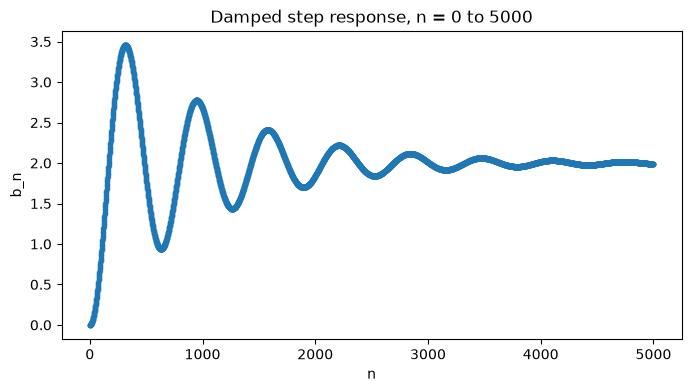
\includegraphics[keepaspectratio]{notebooks/Week03_convergence_files/figure-pdf/cell-7-output-2.png}}

\subsection{Questions to answer before moving
on}\label{questions-to-answer-before-moving-on-1}

\begin{itemize}
\tightlist
\item
  What value does \(b_n\) appear to be converging to? Compare to your
  guess for Dataset 1 --- how did you decide this time, given there's no
  noise to average out?
\item
  Around how many terms does it take before the oscillation dies down to
  something you'd call ``close'' to the limit?
\item
  Pick an \texttt{n} where the plot looks close to the limit, then check
  a later \texttt{n} --- does it ever swing back out? Why might that
  matter for choosing \texttt{N}?
\end{itemize}

\section{\texorpdfstring{Task 4: The \(\varepsilon\) Challenge,
Again}{Task 4: The \textbackslash varepsilon Challenge, Again}}\label{task-4-the-varepsilon-challenge-again}

Same process as Task 2 --- guess \texttt{L\_guess} and \texttt{N\_guess}
for a given \texttt{epsilon}, and check them. The
\texttt{check\_convergence}, \texttt{find\_smallest\_N}, and
\texttt{plot\_challenge} functions from Task 2 work unchanged here; we
just need a table of \(b_n\) values to check against. Since \(b_n\) is
exact (no noise), we can build that table out to a very large \texttt{n}
--- far past where anything interesting happens --- so the check is
effectively verifying ``forever.''

\begin{Shaded}
\begin{Highlighting}[]
\NormalTok{n\_check }\OperatorTok{=}\NormalTok{ np.arange(}\DecValTok{0}\NormalTok{, }\DecValTok{20000}\NormalTok{)      }\CommentTok{\# generous horizon {-}{-} well past where b\_n settles}
\NormalTok{osc\_df }\OperatorTok{=}\NormalTok{ pd.DataFrame(\{}\StringTok{\textquotesingle{}n\textquotesingle{}}\NormalTok{: n\_check, }\StringTok{\textquotesingle{}b\_n\textquotesingle{}}\NormalTok{: b(n\_check)\})}

\CommentTok{\# {-}{-}{-} Your answer {-}{-}{-}}
\NormalTok{EPSILON2 }\OperatorTok{=} \FloatTok{0.08}          \CommentTok{\# \textless{}{-} instructor{-}assigned challenge value}

\NormalTok{L\_guess2 }\OperatorTok{=} \DecValTok{2}          \CommentTok{\# }\AlertTok{TODO}\CommentTok{: your guessed limit}
\NormalTok{N\_guess2 }\OperatorTok{=} \DecValTok{3000}          \CommentTok{\# }\AlertTok{TODO}\CommentTok{: your guessed N}

\NormalTok{check\_convergence(osc\_df, L\_guess2, N\_guess2, EPSILON2, value\_col}\OperatorTok{=}\StringTok{\textquotesingle{}b\_n\textquotesingle{}}\NormalTok{)}
\NormalTok{plot\_challenge(osc\_df, L\_guess2, N\_guess2, EPSILON2, value\_col}\OperatorTok{=}\StringTok{\textquotesingle{}b\_n\textquotesingle{}}\NormalTok{)}
\end{Highlighting}
\end{Shaded}

\begin{verbatim}
✗ Not valid: at n = 3124, |a_n - 2| >= 0.08.
  The sequence leaves the epsilon-band after your N_guess. Try a larger N, or reconsider your L_guess.
\end{verbatim}

\pandocbounded{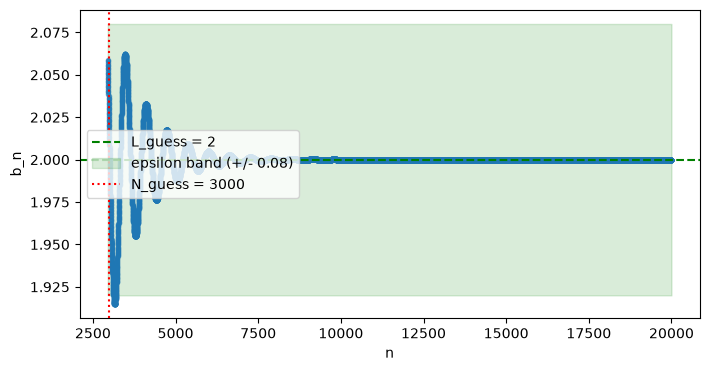
\includegraphics[keepaspectratio]{notebooks/Week03_convergence_files/figure-pdf/cell-8-output-2.png}}

\section{\texorpdfstring{Task 5: Convergence of
\(\sqrt[n]{p}\)}{Task 5: Convergence of \textbackslash sqrt{[}n{]}\{p\}}}\label{task-5-convergence-of-sqrtnp}

Finally, we want to study the convergence behavior of
\(d_n = \sqrt[n]{p}\) for various \(p\). Set the parameters in the cell
below.

\begin{Shaded}
\begin{Highlighting}[]
\CommentTok{\# Set p}
\NormalTok{p }\OperatorTok{=} \DecValTok{2}    \CommentTok{\# Experiment with different p}

\CommentTok{\# Set the range of n you want to consider}
\NormalTok{d\_start }\OperatorTok{=} \DecValTok{1}
\NormalTok{d\_end }\OperatorTok{=} \DecValTok{100}

\KeywordTok{def}\NormalTok{ d(n):}
    \ControlFlowTok{return} \BuiltInTok{float}\NormalTok{(p}\OperatorTok{**}\NormalTok{(}\DecValTok{1}\OperatorTok{/}\NormalTok{n))}
\end{Highlighting}
\end{Shaded}

As above, to return just a single term of the sequence, use
\texttt{d(n)}:

\begin{Shaded}
\begin{Highlighting}[]
\NormalTok{d(}\DecValTok{2}\NormalTok{)}
\end{Highlighting}
\end{Shaded}

\begin{verbatim}
1.4142135623730951
\end{verbatim}

Now let's plot the sequence:

\begin{Shaded}
\begin{Highlighting}[]
\NormalTok{d\_array }\OperatorTok{=}\NormalTok{ np.arange(d\_start, d\_end)}
\NormalTok{d\_vals }\OperatorTok{=}\NormalTok{ p}\OperatorTok{**}\NormalTok{(}\DecValTok{1}\OperatorTok{/}\NormalTok{d\_array)}
\NormalTok{view3 }\OperatorTok{=}\NormalTok{ pd.DataFrame(\{}\StringTok{\textquotesingle{}n\textquotesingle{}}\NormalTok{: d\_array, }\StringTok{\textquotesingle{}d\_n\textquotesingle{}}\NormalTok{: d\_vals\})}
\CommentTok{\# display(view3)}

\NormalTok{plt.figure(figsize}\OperatorTok{=}\NormalTok{(}\DecValTok{8}\NormalTok{, }\DecValTok{4}\NormalTok{))}
\NormalTok{plt.plot(view3[}\StringTok{\textquotesingle{}n\textquotesingle{}}\NormalTok{], view3[}\StringTok{\textquotesingle{}d\_n\textquotesingle{}}\NormalTok{], }\StringTok{\textquotesingle{}.\textquotesingle{}}\NormalTok{, alpha}\OperatorTok{=}\FloatTok{0.7}\NormalTok{)}
\NormalTok{plt.xlabel(}\StringTok{\textquotesingle{}n\textquotesingle{}}\NormalTok{)}
\NormalTok{plt.ylabel(}\StringTok{\textquotesingle{}d\_n\textquotesingle{}}\NormalTok{)}
\NormalTok{plt.title(}\SpecialStringTok{f\textquotesingle{}Sequence n{-}th root of }\SpecialCharTok{\{}\NormalTok{p}\SpecialCharTok{\}}\SpecialStringTok{\textquotesingle{}}\NormalTok{)}
\NormalTok{plt.show()}
\end{Highlighting}
\end{Shaded}

\pandocbounded{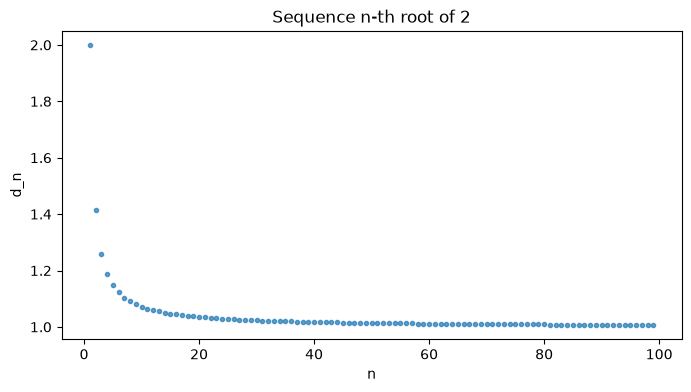
\includegraphics[keepaspectratio]{notebooks/Week03_convergence_files/figure-pdf/cell-11-output-1.png}}

\textbf{Questions:} - Does this sequence converge for all \(p>0\)? - If
so, does the limit depend on \(p\)?

\chapter{Limits of Functions}\label{limits-of-functions}

\begin{tcolorbox}[enhanced jigsaw, arc=.35mm, bottomrule=.15mm, bottomtitle=1mm, breakable, colback=white, colbacktitle=quarto-callout-note-color!10!white, colframe=quarto-callout-note-color-frame, coltitle=black, left=2mm, leftrule=.75mm, opacityback=0, opacitybacktitle=0.6, rightrule=.15mm, title={Companion reading}, titlerule=0mm, toprule=.15mm, toptitle=1mm]

This lecture corresponds to C\&J §1.8 (the concept of limit for a
function of a continuous variable), tying together §1.2.d (continuity)
with the Intermediate Value Theorem of §1.2.e.

\end{tcolorbox}

\section{From Sequences to Functions}\label{from-sequences-to-functions}

We already know what it means for a \emph{sequence} to converge
(Definition~\ref{def-limit}). We now transfer this idea to functions:
instead of asking what happens to \(a_n\) as \(n\to\infty\), we ask what
happens to \(f(x)\) as \(x\) approaches some fixed point \(a\). The
cheapest way to make this precise is to reduce it to something we
already understand --- sequences --- by feeding \emph{every} sequence
approaching \(a\) into \(f\) and demanding that the outputs all converge
to the same value.

\begin{definition}[]\protect\hypertarget{def-function-limit}{}\label{def-function-limit}

\hfill\break
Let \(f\colon D\to\mathbb{R}\) with \(D\subseteq\mathbb{R}\), and let
\(a\in\mathbb{R}\). We say \[
\lim_{x\to a} f(x) = L
\] if for \textbf{every} sequence \((x_n)\) with \(x_n\in D\),
\(x_n\neq a\), and \(x_n\to a\), we have \(f(x_n)\to L\).

\end{definition}

\begin{refremark}
The word ``every'' is doing all the work: it is not enough to find
\emph{some} sequence \(x_n\to a\) with \(f(x_n)\to L\) --- the same
\(L\) must come out no matter which approaching sequence we feed in.
This mirrors uniqueness of sequential limits
(Remark~\ref{rem-limit-unique}): if two different sequences \(x_n\to a\)
and \(x_n'\to a\) produced different outputs \(f(x_n)\to L\) and
\(f(x_n')\to L'\neq L\), the limit \(\lim_{x\to a}f(x)\) would simply
not exist.

\label{rem-function-limit-every-sequence}

\end{refremark}

\begin{example}[]\protect\hypertarget{exm-x-squared-function-limit}{}\label{exm-x-squared-function-limit}

\hfill\break
Let \(f(x) = x^2\). Then \(\displaystyle\lim_{x\to 0} f(x) = 0\).

\begin{proof}
Let \((x_n)\) be an arbitrary sequence with \(x_n\to 0\). We may assume
\(\lvert x_n \rvert\le 1\) for all \(n\) (true eventually, since
\(x_n\to0\)). Then \[
0 \le f(x_n) = x_n^2 \le \lvert x_n \rvert,
\] and \(\lvert x_n \rvert\to 0\), so by the comparison test
(Proposition~\ref{prp-comparison}), \(x_n^2 \to 0\). Since \((x_n)\) was
an arbitrary sequence converging to \(0\),
Definition~\ref{def-function-limit} gives \(\lim_{x\to0} f(x) = 0\).
\end{proof}

\end{example}

\section{\texorpdfstring{The \(\varepsilon\)--\(\delta\)
Version}{The \textbackslash varepsilon--\textbackslash delta Version}}\label{the-varepsilondelta-version}

Just as with continuity (Definition~\ref{def-continuity}), the
sequential definition of a function limit has an equivalent
\(\varepsilon\)--\(\delta\) formulation.

\begin{proposition}[\(\varepsilon\)--\(\delta\) characterization of a
limit]\protect\hypertarget{prp-function-limit-eps-delta}{}\label{prp-function-limit-eps-delta}

Let \(f\colon D\to\mathbb{R}\), \(a\in\mathbb{R}\), \(L\in\mathbb{R}\).
Then \[
\lim_{x\to a} f(x) = L
\] if and only if \[
\text{for every } \varepsilon>0 \text{ there exists } \delta>0 \text{ s.t. }
x\in D,\ 0<\lvert x-a \rvert<\delta \quad \Rightarrow \quad\lvert f(x)-L \rvert<\varepsilon.
\]

\end{proposition}

The proof is the same idea as the equivalence used implicitly for
continuity: if the \(\varepsilon\)--\(\delta\) condition holds and
\(x_n\to a\), choosing \(N\) so that \(\lvert x_n-a \rvert<\delta\) for
\(n\ge N\) forces \(\lvert f(x_n)-L \rvert<\varepsilon\) for \(n\ge N\),
i.e.~\(f(x_n)\to L\). Conversely, if the \(\varepsilon\)--\(\delta\)
condition \emph{fails} for some \(\varepsilon>0\), then for every
\(\delta = \tfrac1n\) we can pick a point \(x_n\) with
\(0<\lvert x_n-a \rvert<\tfrac1n\) but
\(\lvert f(x_n)-L \rvert\ge\varepsilon\) --- producing a sequence
\(x_n\to a\) with \(f(x_n)\not\to L\), so the sequential definition
fails too.

The only difference from Definition~\ref{def-continuity} is the
punctured condition \(0<\lvert x-a \rvert\): a limit does not care what
happens (or fails to happen) \emph{at} \(a\) itself, only nearby. This
is what lets us connect the two notions.

\begin{proposition}[Continuity,
restated]\protect\hypertarget{prp-continuity-via-limit}{}\label{prp-continuity-via-limit}

Let \(f\colon D\to\mathbb{R}\) and \(a\in D\). Then \(f\) is continuous
at \(a\) (Definition~\ref{def-continuity}) if and only if \[
\lim_{x\to a} f(x) \text{ exists and equals } f(a).
\]

\end{proposition}

This is exactly Definition~\ref{def-continuity} with the roles of \(x\)
and \(a\) relabeled: continuity says
\(\lvert x-a \rvert<\delta \quad \Rightarrow \quad\lvert f(x)-f(a) \rvert<\varepsilon\),
which is the \(\varepsilon\)--\(\delta\) condition of
Proposition~\ref{prp-function-limit-eps-delta} with \(L=f(a)\) (the
point \(x=a\) itself trivially satisfies
\(\lvert f(x)-f(a) \rvert=0<\varepsilon\), so punctured and unpunctured
versions agree once \(L=f(a)\)).

\section{Examples}\label{examples}

\begin{example}[]\protect\hypertarget{exm-cube-continuous}{}\label{exm-cube-continuous}

\hfill\break
\(f(x) = x^3\) is continuous at every \(a\in\mathbb{R}\).

\begin{proof}
Let \(x_n\to a\). By the limit laws for sequences
(Proposition~\ref{prp-limit-laws}), \[
x_n^3 = x_n\cdot x_n\cdot x_n \longrightarrow a\cdot a\cdot a = a^3.
\] Hence \(f(x_n)\to f(a)\) for every sequence \(x_n\to a\), so
\(\lim_{x\to a} f(x) = f(a)\), and
Proposition~\ref{prp-continuity-via-limit} gives continuity at \(a\).
\end{proof}

\end{example}

\begin{example}[]\protect\hypertarget{exm-dirichlet-discontinuous}{}\label{exm-dirichlet-discontinuous}

\hfill\break
The \textbf{Dirichlet function} \[
f(x) = \begin{cases} 1 & x\in\mathbb{Q}\\ 0 & x\notin\mathbb{Q}\end{cases}
\] is discontinuous at every \(a\in\mathbb{R}\).

Take \(a=1\). Consider the two sequences \[
x_n = 1+\frac1n \quad(\text{rational}), \qquad\qquad y_n = 1+\frac{\sqrt2}{n} \quad(\text{irrational}).
\] Both converge to \(1\), but \[
f(x_n) \equiv 1 \to 1, \qquad\qquad f(y_n) \equiv 0 \to 0 \neq f(1) = 1.
\] Since two sequences converging to \(a=1\) produce different limits
for \(f\), \(\lim_{x\to1}f(x)\) does not exist
(Remark~\ref{rem-function-limit-every-sequence}), so \(f\) is not
continuous at \(1\).

\end{example}

\begin{exercise}[]\protect\hypertarget{exr-dirichlet-general-a}{}\label{exr-dirichlet-general-a}

Adapt the argument of Example~\ref{exm-dirichlet-discontinuous} to an
arbitrary \(a\in\mathbb{R}\): exhibit a rational sequence and an
irrational sequence, both converging to \(a\), on which the Dirichlet
function takes different limiting values. Conclude that \(f\) is
discontinuous at \emph{every} \(a\in\mathbb{R}\).

\end{exercise}

\begin{example}[]\protect\hypertarget{exm-piecewise-jump}{}\label{exm-piecewise-jump}

\hfill\break
Let \[
f(x) = \begin{cases} x^3+16 & x<0 \\ -2x+3 & x\ge 0. \end{cases}
\] Take \(x_n = -\tfrac1n \to 0\). Then \[
f(x_n) = \left(-\frac1n\right)^{\!3} + 16 \longrightarrow 16 \neq f(0) = 3,
\] so \(f\) is discontinuous at \(0\). We will see below exactly what
kind of discontinuity this is.

\end{example}

\section{One-Sided Limits}\label{one-sided-limits}

For Example~\ref{exm-piecewise-jump}, the failure of continuity comes
from the two ``branches'' of \(f\) disagreeing at \(0\) --- approaching
from the left gives a different answer than approaching from the right.
To capture this we restrict which sequences \(x_n\to a\) we are allowed
to test with.

\begin{definition}[]\protect\hypertarget{def-one-sided-limits}{}\label{def-one-sided-limits}

\hfill\break
Let \(f\colon D\to\mathbb{R}\) and \(a\in\mathbb{R}\).

\begin{itemize}
\tightlist
\item
  \(\displaystyle\lim_{x\to a^-} f(x) = L\) (the \textbf{left-sided
  limit}) if \(f(x_n)\to L\) for every \emph{increasing} sequence
  \(x_n \nearrow a\) with \(x_n\in D\).
\item
  \(\displaystyle\lim_{x\to a^+} f(x) = L\) (the \textbf{right-sided
  limit}) if \(f(x_n)\to L\) for every \emph{decreasing} sequence
  \(x_n \searrow a\) with \(x_n\in D\).
\end{itemize}

\end{definition}

\begin{refremark}
The left- and right-sided limits may disagree. For \(f\) as in
Example~\ref{exm-piecewise-jump}, \[
\lim_{x\to0^-} f(x) = 16, \qquad\qquad \lim_{x\to0^+} f(x) = 3,
\] since \(x^3+16\to16\) along any \(x_n\nearrow0\), while \(-2x+3\to3\)
along any \(x_n\searrow0\).

\label{rem-one-sided-disagree}

\end{refremark}

\begin{definition}[]\protect\hypertarget{def-jump-discontinuity}{}\label{def-jump-discontinuity}

\hfill\break
\(f\) has a \textbf{jump discontinuity} at \(a\) if both one-sided
limits exist and are finite, but \[
\lim_{x\to a^-} f(x) \neq \lim_{x\to a^+} f(x).
\] This makes precise the informal description from
Remark~\ref{rem-jump-discontinuity}, and excludes the unbounded case of
Remark~\ref{rem-infinite-discontinuity}, where no finite one-sided limit
exists at all. The function of Example~\ref{exm-piecewise-jump} has a
jump discontinuity at \(0\).

\end{definition}

\begin{theorem}[]\protect\hypertarget{thm-continuity-one-sided}{}\label{thm-continuity-one-sided}

\hfill\break
Let \(f\colon D\to\mathbb{R}\) and \(a\in D\). Then \(f\) is continuous
at \(a\) if and only if \[
\lim_{x\to a^-} f(x) = f(a) = \lim_{x\to a^+} f(x).
\]

\end{theorem}

Like the two-sided limit
(Proposition~\ref{prp-function-limit-eps-delta}), each one-sided limit
has an equivalent \(\varepsilon\)--\(\delta\) form obtained by
restricting to one side: \[
\lim_{x\to a^-} f(x) = L \quad \Leftrightarrow \quad\forall\varepsilon>0\ \exists\delta>0:\ a-\delta<x<a \quad \Rightarrow \quad\lvert f(x)-L \rvert<\varepsilon,
\] and symmetrically for \(\lim_{x\to a^+}f(x)=L\) with
\(a<x<a+\delta\).

\begin{proof}
If \(f\) is continuous at \(a\), then \(f(x_n)\to f(a)\) for
\emph{every} sequence \(x_n\to a\)
(Proposition~\ref{prp-continuity-via-limit}) --- in particular for every
increasing sequence \(x_n\nearrow a\) and every decreasing sequence
\(x_n\searrow a\), giving both one-sided limits equal to \(f(a)\).

Conversely, suppose both one-sided limits equal \(f(a)\), and let
\(\varepsilon>0\). By the \(\varepsilon\)--\(\delta\) forms above there
exist \(\delta_1,\delta_2>0\) with \[
a-\delta_1<x<a \quad \Rightarrow \quad\lvert f(x)-f(a) \rvert<\varepsilon, \qquad\qquad a<x<a+\delta_2 \quad \Rightarrow \quad\lvert f(x)-f(a) \rvert<\varepsilon.
\] Let \(\delta=\min(\delta_1,\delta_2)\). If
\(0<\lvert x-a \rvert<\delta\), then either \(a-\delta<x<a\) or
\(a<x<a+\delta\), so in both cases
\(\lvert f(x)-f(a) \rvert<\varepsilon\); and \(x=a\) trivially gives
\(\lvert f(x)-f(a) \rvert=0<\varepsilon\). So
\(\lvert x-a \rvert<\delta \quad \Rightarrow \quad\lvert f(x)-f(a) \rvert<\varepsilon\),
which is exactly Definition~\ref{def-continuity}.
\end{proof}

\section{Limit Laws for Functions}\label{limit-laws-for-functions}

Because Definition~\ref{def-function-limit} reduces everything to
sequences, the arithmetic of function limits carries over directly from
the arithmetic of sequence limits (Proposition~\ref{prp-limit-laws}).

\begin{proposition}[Arithmetic of function
limits]\protect\hypertarget{prp-function-limit-laws}{}\label{prp-function-limit-laws}

Suppose \(\lim_{x\to a} f(x) = L\) and \(\lim_{x\to a} g(x) = M\). Then
\[
\lim_{x\to a} \big(f(x)+g(x)\big) = L+M, \qquad\qquad \lim_{x\to a} f(x)g(x) = LM,
\] and, if \(M\neq0\), \[
\lim_{x\to a} \frac{f(x)}{g(x)} = \frac{L}{M}.
\]

\end{proposition}

\begin{corollary}[]\protect\hypertarget{cor-continuity-algebra}{}\label{cor-continuity-algebra}

If \(a\in\operatorname{dom}(f)\cap\operatorname{dom}(g)\) and \(f,g\)
are continuous at \(a\), then \(f+g\), \(f\cdot g\), and (provided
\(g(a)\neq0\)) \(f/g\) are continuous at \(a\).

\end{corollary}

\begin{example}[]\protect\hypertarget{exm-rational-function-limit}{}\label{exm-rational-function-limit}

\hfill\break
\[
\lim_{x\to 0} \frac{x^3-3x+4}{x^2+\cos(x)}
= \frac{\lim_{x\to0}x^3 - \lim_{x\to0}3x + \lim_{x\to0}4}{\lim_{x\to0}x^2 + \lim_{x\to0}\cos(x)}
= \frac{0-0+4}{0+1} = 4.
\]

\end{example}

\begin{example}[]\protect\hypertarget{exm-quotient-careful}{}\label{exm-quotient-careful}

\hfill\break
\textbf{Careful:} the quotient rule requires the \emph{denominator's}
limit to be nonzero --- it says nothing when both numerator and
denominator vanish. For \[
\lim_{x\to a} \frac{x^2-a^2}{x-a},
\] we have \(\lim_{x\to a}(x-a) = 0\), so
Proposition~\ref{prp-function-limit-laws} simply does not apply.
Instead, factor first: \[
\frac{x^2-a^2}{x-a} = \frac{(x-a)(x+a)}{x-a} = x+a \qquad (x\neq a),
\] and only \emph{then} take the limit: \(\lim_{x\to a}(x+a) = 2a\).

\end{example}

\section{Continuity of Combinations and
Compositions}\label{continuity-of-combinations-and-compositions}

Proposition~\ref{prp-continuity-via-limit} lets us move freely between
``\(f\) is continuous at \(a\)'' and ``\(\lim_{x\to
a}f(x)=f(a)\)''. The next fact is the one we have already been using
informally whenever we wrote something like
\(\lim_{x\to a}\cos(h(x)) = \cos\!\big(\lim_{x\to a}h(x)\big)\): a limit
may be passed from the \emph{outside} of a continuous function to its
\emph{inside}.

\begin{proposition}[Limits pass through continuous
functions]\protect\hypertarget{prp-limit-inside-continuous}{}\label{prp-limit-inside-continuous}

Suppose \(\lim_{x\to a} f(x) = L\), and \(g\) is continuous at \(L\).
Then \[
\lim_{x\to a} g(f(x)) = g(L) = g\Big(\lim_{x\to a} f(x)\Big).
\]

\end{proposition}

\begin{proof}
Let \((x_n)\) be an arbitrary sequence with
\(x_n\in\operatorname{dom}(f)\), \(x_n\neq a\), \(x_n\to a\). By
hypothesis (Definition~\ref{def-function-limit}), \(f(x_n)\to L\). Since
\(g\) is continuous at \(L\), feeding the sequence
\(\big(f(x_n)\big)\to L\) into Definition~\ref{def-continuity} gives
\(g(f(x_n))\to g(L)\). As \((x_n)\) was an arbitrary sequence
approaching \(a\), Definition~\ref{def-function-limit} gives
\(\lim_{x\to a}g(f(x)) = g(L)\).
\end{proof}

Taking \(L=f(a)\) recovers continuity of a composition:

\begin{corollary}[Continuity of
compositions]\protect\hypertarget{cor-continuity-composition}{}\label{cor-continuity-composition}

If \(f\) is continuous at \(a\) and \(g\) is continuous at \(f(a)\),
then \(g\circ f\) is continuous at \(a\).

\end{corollary}

\begin{proof}
Since \(f\) is continuous at \(a\),
Proposition~\ref{prp-continuity-via-limit} gives
\(\lim_{x\to a}f(x) = f(a)\). Applying
Proposition~\ref{prp-limit-inside-continuous} with \(L=f(a)\), \[
\lim_{x\to a} (g\circ f)(x) = \lim_{x\to a} g(f(x)) = g(f(a)) = (g\circ f)(a),
\] so \(g\circ f\) is continuous at \(a\) by
Proposition~\ref{prp-continuity-via-limit}.
\end{proof}

Together with Corollary~\ref{cor-continuity-algebra} --- continuity of
\(f+g\), \(f\cdot g\), and \(f/g\) (where \(g\neq0\)) from continuity of
\(f\) and \(g\) --- Corollary~\ref{cor-continuity-composition} means
that \emph{any} function built out of continuous building blocks by
finitely many arithmetic operations and compositions is again continuous
wherever it is defined. This is exactly the justification behind phrases
like ``combination of continuous functions'' or ``composition of
continuous functions'' used to evaluate a limit by plugging in, as in
Example~\ref{exm-rational-function-limit} above.

\begin{refremark}
The \hyperref[the-elementary-functions]{elementary functions} ---
polynomials, rational functions, power and algebraic functions,
exponentials, logarithms, and the trigonometric functions --- are
continuous at every point of their domain. Each basic type can be
checked directly from Definition~\ref{def-continuity}, the way we
checked \(x^3\) in Example~\ref{exm-cube-continuous};
Corollary~\ref{cor-continuity-algebra} and
Corollary~\ref{cor-continuity-composition} then extend continuity to
every function assembled from these by arithmetic and composition, such
as \(\sqrt{2+\sqrt{2x}}\) or \(\cos\!\big(\pi\sin(x)/x\big)\). Once we
develop differentiation, this will also follow a second way: every
elementary function is differentiable wherever it is defined, and
differentiability will turn out to imply continuity.

\label{rem-elementary-continuous}

\end{refremark}

\section{The Intermediate Value
Theorem}\label{the-intermediate-value-theorem}

\begin{theorem}[Intermediate Value
Theorem]\protect\hypertarget{thm-ivt}{}\label{thm-ivt}

Let \(f\colon\mathbb{R}\to\mathbb{R}\) be continuous, and suppose
\(a<b\) with \(f(a)<0\) and \(f(b)>0\). Then there exists \(c\in(a,b)\)
with \(f(c)=0\).

\end{theorem}

\begin{proof}
We construct \(c\) by \textbf{bisection}. Set \(a_1=a\), \(b_1=b\), so
\(f(a_1)\le0\le f(b_1)\). Given \(a_n,b_n\) with \(f(a_n)\le0\) and
\(f(b_n)\ge0\), let \(m_n = \tfrac{a_n+b_n}{2}\).

\begin{itemize}
\tightlist
\item
  If \(f(m_n)=0\), we are done --- take \(c=m_n\).
\item
  If \(f(m_n)<0\), set \(a_{n+1}=m_n\), \(b_{n+1}=b_n\).
\item
  If \(f(m_n)>0\), set \(a_{n+1}=a_n\), \(b_{n+1}=m_n\).
\end{itemize}

In either of the last two cases \(f(a_{n+1})\le0\le f(b_{n+1})\), so the
invariant is preserved, and we continue. If the process never
terminates, this produces sequences with \((a_n)\) increasing, \((b_n)\)
decreasing, \(a_n\le b_n\) for all \(n\), and \[
b_n - a_n = \frac{b-a}{2^{n-1}} \longrightarrow 0
\] (the interval length halves at each step; compare
Exercise~\ref{exr-warmup-half-n}). By
Corollary~\ref{cor-monotone-squeeze}, \((a_n)\) and \((b_n)\) converge
to a common limit \(c\in[a,b]\).

Since \(f\) is continuous, Proposition~\ref{prp-continuity-via-limit}
gives \(f(a_n)\to f(c)\) and \(f(b_n)\to f(c)\). Now \(f(a_n)\le0\) for
every \(n\); if we had \(f(c)>0\), taking \(\varepsilon=f(c)/2\) in the
definition of convergence would force \(f(a_n)>f(c)/2>0\) for large
\(n\), a contradiction. So \(f(c)\le0\). The same argument with
\(f(b_n)\ge0\) gives \(f(c)\ge0\). Hence \(f(c)=0\), and \(a<c<b\) since
\(f(a)<0\) and \(f(b)>0\) rule out \(c=a\) or \(c=b\).
\end{proof}

\begin{refremark}
The same bisection idea proves the more general statement: if \(f\) is
continuous on \([a,b]\) and \(y\) lies between \(f(a)\) and \(f(b)\),
then \(f(c)=y\) for some \(c\in[a,b]\) --- apply Theorem~\ref{thm-ivt}
to \(f(x)-y\).

\label{rem-ivt-general}

\end{refremark}

\section{Summary}\label{summary-6}

\begin{itemize}
\tightlist
\item
  \(\displaystyle\lim_{x\to a} f(x) = L\)
  (Definition~\ref{def-function-limit}) means \(f(x_n)\to L\) for
  \textbf{every} sequence \(x_n\to a\) in \(\operatorname{dom}(f)\) ---
  this reduces function limits to sequence limits, and is equivalent to
  the \(\varepsilon\)--\(\delta\) condition of
  Proposition~\ref{prp-function-limit-eps-delta}.
\item
  \textbf{Continuity restated:} \(f\) is continuous at \(a\) exactly
  when \(\lim_{x\to a}f(x)\) exists and equals \(f(a)\)
  (Proposition~\ref{prp-continuity-via-limit}).
\item
  \textbf{One-sided limits} (Definition~\ref{def-one-sided-limits}) test
  only monotone sequences approaching from one side. A \textbf{jump
  discontinuity} (Definition~\ref{def-jump-discontinuity}) is exactly a
  point where both one-sided limits exist (finitely) but disagree; \(f\)
  is continuous at \(a\) iff both one-sided limits equal \(f(a)\)
  (Theorem~\ref{thm-continuity-one-sided}).
\item
  The \textbf{limit laws} (Proposition~\ref{prp-function-limit-laws})
  compute limits of sums, products, and quotients termwise, and give
  continuity of \(f+g\), \(f\cdot g\), \(f/g\) from continuity of \(f\)
  and \(g\) (Corollary~\ref{cor-continuity-algebra}) --- but a
  \(\tfrac00\) form must be simplified \emph{before} the quotient rule
  applies (Example~\ref{exm-quotient-careful}).
\item
  \textbf{Compositions of continuous functions are continuous}
  (Corollary~\ref{cor-continuity-composition}), and more generally a
  limit may be passed through a continuous function from the outside in
  (Proposition~\ref{prp-limit-inside-continuous}). Together with the
  arithmetic rule above, this shows every \textbf{elementary function}
  is continuous where defined (Remark~\ref{rem-elementary-continuous}).
\item
  The \textbf{Intermediate Value Theorem} (Theorem~\ref{thm-ivt}): a
  continuous function that is negative at \(a\) and positive at \(b\)
  must vanish somewhere in between. The proof bisects \([a,b]\) into
  nested intervals shrinking to a point \(c\), then uses continuity to
  pass \(f(a_n)\le0\le f(b_n)\) to the limit.
\end{itemize}




\end{document}
